\documentclass[12pt,a4paper,]{book}
\def\ifdoblecara{} %% set to true
\def\ifprincipal{} %% set to true
\def\ifcitapandoc{} %% set to true
\let\ifcitapandoc\undefined %% set to false
\usepackage{lmodern}
% sin fontmathfamily
\usepackage{amssymb,amsmath}
\usepackage{ifxetex,ifluatex}
%\usepackage{fixltx2e} % provides \textsubscript %PLLC
\ifnum 0\ifxetex 1\fi\ifluatex 1\fi=0 % if pdftex
  \usepackage[T1]{fontenc}
  \usepackage[utf8]{inputenc}
\else % if luatex or xelatex
  \ifxetex
    \usepackage{mathspec}
  \else
    \usepackage{fontspec}
  \fi
  \defaultfontfeatures{Ligatures=TeX,Scale=MatchLowercase}
\fi
% use upquote if available, for straight quotes in verbatim environments
\IfFileExists{upquote.sty}{\usepackage{upquote}}{}
% use microtype if available
\IfFileExists{microtype.sty}{%
\usepackage{microtype}
\UseMicrotypeSet[protrusion]{basicmath} % disable protrusion for tt fonts
}{}
\usepackage[margin=2.5cm]{geometry}
\usepackage{hyperref}
\hypersetup{unicode=true,
              pdfborder={0 0 0},
              breaklinks=true}
\urlstyle{same}  % don't use monospace font for urls
%
\usepackage[usenames,dvipsnames]{xcolor}  %new PLLC
\usepackage{color}
\usepackage{fancyvrb}
\newcommand{\VerbBar}{|}
\newcommand{\VERB}{\Verb[commandchars=\\\{\}]}
\DefineVerbatimEnvironment{Highlighting}{Verbatim}{commandchars=\\\{\}}
% Add ',fontsize=\small' for more characters per line
\usepackage{framed}
\definecolor{shadecolor}{RGB}{248,248,248}
\newenvironment{Shaded}{\begin{snugshade}}{\end{snugshade}}
\newcommand{\AlertTok}[1]{\textcolor[rgb]{0.94,0.16,0.16}{#1}}
\newcommand{\AnnotationTok}[1]{\textcolor[rgb]{0.56,0.35,0.01}{\textbf{\textit{#1}}}}
\newcommand{\AttributeTok}[1]{\textcolor[rgb]{0.13,0.29,0.53}{#1}}
\newcommand{\BaseNTok}[1]{\textcolor[rgb]{0.00,0.00,0.81}{#1}}
\newcommand{\BuiltInTok}[1]{#1}
\newcommand{\CharTok}[1]{\textcolor[rgb]{0.31,0.60,0.02}{#1}}
\newcommand{\CommentTok}[1]{\textcolor[rgb]{0.56,0.35,0.01}{\textit{#1}}}
\newcommand{\CommentVarTok}[1]{\textcolor[rgb]{0.56,0.35,0.01}{\textbf{\textit{#1}}}}
\newcommand{\ConstantTok}[1]{\textcolor[rgb]{0.56,0.35,0.01}{#1}}
\newcommand{\ControlFlowTok}[1]{\textcolor[rgb]{0.13,0.29,0.53}{\textbf{#1}}}
\newcommand{\DataTypeTok}[1]{\textcolor[rgb]{0.13,0.29,0.53}{#1}}
\newcommand{\DecValTok}[1]{\textcolor[rgb]{0.00,0.00,0.81}{#1}}
\newcommand{\DocumentationTok}[1]{\textcolor[rgb]{0.56,0.35,0.01}{\textbf{\textit{#1}}}}
\newcommand{\ErrorTok}[1]{\textcolor[rgb]{0.64,0.00,0.00}{\textbf{#1}}}
\newcommand{\ExtensionTok}[1]{#1}
\newcommand{\FloatTok}[1]{\textcolor[rgb]{0.00,0.00,0.81}{#1}}
\newcommand{\FunctionTok}[1]{\textcolor[rgb]{0.13,0.29,0.53}{\textbf{#1}}}
\newcommand{\ImportTok}[1]{#1}
\newcommand{\InformationTok}[1]{\textcolor[rgb]{0.56,0.35,0.01}{\textbf{\textit{#1}}}}
\newcommand{\KeywordTok}[1]{\textcolor[rgb]{0.13,0.29,0.53}{\textbf{#1}}}
\newcommand{\NormalTok}[1]{#1}
\newcommand{\OperatorTok}[1]{\textcolor[rgb]{0.81,0.36,0.00}{\textbf{#1}}}
\newcommand{\OtherTok}[1]{\textcolor[rgb]{0.56,0.35,0.01}{#1}}
\newcommand{\PreprocessorTok}[1]{\textcolor[rgb]{0.56,0.35,0.01}{\textit{#1}}}
\newcommand{\RegionMarkerTok}[1]{#1}
\newcommand{\SpecialCharTok}[1]{\textcolor[rgb]{0.81,0.36,0.00}{\textbf{#1}}}
\newcommand{\SpecialStringTok}[1]{\textcolor[rgb]{0.31,0.60,0.02}{#1}}
\newcommand{\StringTok}[1]{\textcolor[rgb]{0.31,0.60,0.02}{#1}}
\newcommand{\VariableTok}[1]{\textcolor[rgb]{0.00,0.00,0.00}{#1}}
\newcommand{\VerbatimStringTok}[1]{\textcolor[rgb]{0.31,0.60,0.02}{#1}}
\newcommand{\WarningTok}[1]{\textcolor[rgb]{0.56,0.35,0.01}{\textbf{\textit{#1}}}}

% PLLC modifica-ini
% PLLC modifica-fin

\IfFileExists{parskip.sty}{%
\usepackage{parskip}
}{% else
\setlength{\parindent}{0pt}
\setlength{\parskip}{6pt plus 2pt minus 1pt}
}
\setlength{\emergencystretch}{3em}  % prevent overfull lines
\providecommand{\tightlist}{%
  \setlength{\itemsep}{0pt}\setlength{\parskip}{0pt}}
\setcounter{secnumdepth}{5}
% Redefines (sub)paragraphs to behave more like sections
\ifx\paragraph\undefined\else
\let\oldparagraph\paragraph
\renewcommand{\paragraph}[1]{\oldparagraph{#1}\mbox{}}
\fi
\ifx\subparagraph\undefined\else
\let\oldsubparagraph\subparagraph
\renewcommand{\subparagraph}[1]{\oldsubparagraph{#1}\mbox{}}
\fi

%%% Use protect on footnotes to avoid problems with footnotes in titles
\let\rmarkdownfootnote\footnote%
\def\footnote{\protect\rmarkdownfootnote}


  \title{}
    \author{}
    \date{}
  

%%%%%%% inicio: latex_preambulo.tex PLLC


%% UTILIZA CODIFICACIÓN UTF-8
%% MODIFICARLO CONVENIENTEMENTE PARA USARLO CON OTRAS CODIFICACIONES


%\usepackage[spanish,es-nodecimaldot,es-noshorthands]{babel}
\usepackage[spanish,es-nodecimaldot,es-noshorthands,es-tabla]{babel}
% Ver: es-tabla (en: https://osl.ugr.es/CTAN/macros/latex/contrib/babel-contrib/spanish/spanish.pdf)
% es-tabla (en: https://tex.stackexchange.com/questions/80443/change-the-word-table-in-table-captions)
\usepackage[spanish, plain, datebegin,sortcompress,nocomment,
noabstract]{flexbib}
 
\usepackage{float}
\usepackage{placeins}
\usepackage{fancyhdr}
% Solucion: ! LaTeX Error: Command \counterwithout already defined.
% https://tex.stackexchange.com/questions/425600/latex-error-command-counterwithout-already-defined
\let\counterwithout\relax
\let\counterwithin\relax
\usepackage{chngcntr}
%\usepackage{microtype}  %antes en template PLLC
\usepackage[utf8]{inputenc}
\usepackage[T1]{fontenc} % Usa codificación 8-bit que tiene 256 glyphs

%\usepackage[dvipsnames]{xcolor}
%\usepackage[usenames,dvipsnames]{xcolor}  %new
\usepackage{pdfpages}
%\usepackage{natbib}




% Para portada: latex_paginatitulo_mod_ST02.tex (inicio)
\usepackage{tikz}
\usepackage{epigraph}
\input{portadas/latex_paginatitulo_mod_ST02_add.sty}
% Para portada: latex_paginatitulo_mod_ST02.tex (fin)

% Para portada: latex_paginatitulo_mod_OV01.tex (inicio)
\usepackage{cpimod}
% Para portada: latex_paginatitulo_mod_OV01.tex (fin)

% Para portada: latex_paginatitulo_mod_OV03.tex (inicio)
\usepackage{KTHEEtitlepage}
% Para portada: latex_paginatitulo_mod_OV03.tex (fin)

\renewcommand{\contentsname}{Índice}
\renewcommand{\listfigurename}{Índice de figuras}
\renewcommand{\listtablename}{Índice de tablas}
\newcommand{\bcols}{}
\newcommand{\ecols}{}
\newcommand{\bcol}[1]{\begin{minipage}{#1\linewidth}}
\newcommand{\ecol}{\end{minipage}}
\newcommand{\balertblock}[1]{\begin{alertblock}{#1}}
\newcommand{\ealertblock}{\end{alertblock}}
\newcommand{\bitemize}{\begin{itemize}}
\newcommand{\eitemize}{\end{itemize}}
\newcommand{\benumerate}{\begin{enumerate}}
\newcommand{\eenumerate}{\end{enumerate}}
\newcommand{\saltopagina}{\newpage}
\newcommand{\bcenter}{\begin{center}}
\newcommand{\ecenter}{\end{center}}
\newcommand{\beproof}{\begin{proof}} %new
\newcommand{\eeproof}{\end{proof}} %new
%De: https://texblog.org/2007/11/07/headerfooter-in-latex-with-fancyhdr/
% \fancyhead
% E: Even page
% O: Odd page
% L: Left field
% C: Center field
% R: Right field
% H: Header
% F: Footer
%\fancyhead[CO,CE]{Resultados}

%OPCION 1
% \fancyhead[LE,RO]{\slshape \rightmark}
% \fancyhead[LO,RE]{\slshape \leftmark}
% \fancyfoot[C]{\thepage}
% \renewcommand{\headrulewidth}{0.4pt}
% \renewcommand{\footrulewidth}{0pt}

%OPCION 2
% \fancyhead[LE,RO]{\slshape \rightmark}
% \fancyfoot[LO,RE]{\slshape \leftmark}
% \fancyfoot[LE,RO]{\thepage}
% \renewcommand{\headrulewidth}{0.4pt}
% \renewcommand{\footrulewidth}{0.4pt}
%%%%%%%%%%
\usepackage{calc,amsfonts}
% Elimina la cabecera de páginas impares vacías al finalizar los capítulos
\usepackage{emptypage}
\makeatletter

%\definecolor{ocre}{RGB}{25,25,243} % Define el color azul (naranja) usado para resaltar algunas salidas
\definecolor{ocre}{RGB}{0,0,0} % Define el color a negro (aparece en los teoremas

%\usepackage{calc} 


%era if(csl-refs) con dolares
% metodobib: true


\usepackage{lipsum}

%\usepackage{tikz} % Requerido para dibujar formas personalizadas

%\usepackage{amsmath,amsthm,amssymb,amsfonts}
\usepackage{amsthm}


% Boxed/framed environments
\newtheoremstyle{ocrenumbox}% % Theorem style name
{0pt}% Space above
{0pt}% Space below
{\normalfont}% % Body font
{}% Indent amount
{\small\bf\sffamily\color{ocre}}% % Theorem head font
{\;}% Punctuation after theorem head
{0.25em}% Space after theorem head
{\small\sffamily\color{ocre}\thmname{#1}\nobreakspace\thmnumber{\@ifnotempty{#1}{}\@upn{#2}}% Theorem text (e.g. Theorem 2.1)
\thmnote{\nobreakspace\the\thm@notefont\sffamily\bfseries\color{black}---\nobreakspace#3.}} % Optional theorem note
\renewcommand{\qedsymbol}{$\blacksquare$}% Optional qed square

\newtheoremstyle{blacknumex}% Theorem style name
{5pt}% Space above
{5pt}% Space below
{\normalfont}% Body font
{} % Indent amount
{\small\bf\sffamily}% Theorem head font
{\;}% Punctuation after theorem head
{0.25em}% Space after theorem head
{\small\sffamily{\tiny\ensuremath{\blacksquare}}\nobreakspace\thmname{#1}\nobreakspace\thmnumber{\@ifnotempty{#1}{}\@upn{#2}}% Theorem text (e.g. Theorem 2.1)
\thmnote{\nobreakspace\the\thm@notefont\sffamily\bfseries---\nobreakspace#3.}}% Optional theorem note

\newtheoremstyle{blacknumbox} % Theorem style name
{0pt}% Space above
{0pt}% Space below
{\normalfont}% Body font
{}% Indent amount
{\small\bf\sffamily}% Theorem head font
{\;}% Punctuation after theorem head
{0.25em}% Space after theorem head
{\small\sffamily\thmname{#1}\nobreakspace\thmnumber{\@ifnotempty{#1}{}\@upn{#2}}% Theorem text (e.g. Theorem 2.1)
\thmnote{\nobreakspace\the\thm@notefont\sffamily\bfseries---\nobreakspace#3.}}% Optional theorem note

% Non-boxed/non-framed environments
\newtheoremstyle{ocrenum}% % Theorem style name
{5pt}% Space above
{5pt}% Space below
{\normalfont}% % Body font
{}% Indent amount
{\small\bf\sffamily\color{ocre}}% % Theorem head font
{\;}% Punctuation after theorem head
{0.25em}% Space after theorem head
{\small\sffamily\color{ocre}\thmname{#1}\nobreakspace\thmnumber{\@ifnotempty{#1}{}\@upn{#2}}% Theorem text (e.g. Theorem 2.1)
\thmnote{\nobreakspace\the\thm@notefont\sffamily\bfseries\color{black}---\nobreakspace#3.}} % Optional theorem note
\renewcommand{\qedsymbol}{$\blacksquare$}% Optional qed square
\makeatother



% Define el estilo texto theorem para cada tipo definido anteriormente
\newcounter{dummy} 
\numberwithin{dummy}{section}
\theoremstyle{ocrenumbox}
\newtheorem{theoremeT}[dummy]{Teorema}  % (Pedro: Theorem)
\newtheorem{problem}{Problema}[chapter]  % (Pedro: Problem)
\newtheorem{exerciseT}{Ejercicio}[chapter] % (Pedro: Exercise)
\theoremstyle{blacknumex}
\newtheorem{exampleT}{Ejemplo}[chapter] % (Pedro: Example)
\theoremstyle{blacknumbox}
\newtheorem{vocabulary}{Vocabulario}[chapter]  % (Pedro: Vocabulary)
\newtheorem{definitionT}{Definición}[section]  % (Pedro: Definition)
\newtheorem{corollaryT}[dummy]{Corolario}  % (Pedro: Corollary)
\theoremstyle{ocrenum}
\newtheorem{proposition}[dummy]{Proposición} % (Pedro: Proposition)


\usepackage[framemethod=default]{mdframed}



\newcommand{\intoo}[2]{\mathopen{]}#1\,;#2\mathclose{[}}
\newcommand{\ud}{\mathop{\mathrm{{}d}}\mathopen{}}
\newcommand{\intff}[2]{\mathopen{[}#1\,;#2\mathclose{]}}
\newtheorem{notation}{Notation}[chapter]


\mdfdefinestyle{exampledefault}{%
rightline=true,innerleftmargin=10,innerrightmargin=10,
frametitlerule=true,frametitlerulecolor=green,
frametitlebackgroundcolor=yellow,
frametitlerulewidth=2pt}


% Theorem box
\newmdenv[skipabove=7pt,
skipbelow=7pt,
backgroundcolor=black!5,
linecolor=ocre,
innerleftmargin=5pt,
innerrightmargin=5pt,
innertopmargin=10pt,%5pt
leftmargin=0cm,
rightmargin=0cm,
innerbottommargin=5pt]{tBox}

% Exercise box	  
\newmdenv[skipabove=7pt,
skipbelow=7pt,
rightline=false,
leftline=true,
topline=false,
bottomline=false,
backgroundcolor=ocre!10,
linecolor=ocre,
innerleftmargin=5pt,
innerrightmargin=5pt,
innertopmargin=10pt,%5pt
innerbottommargin=5pt,
leftmargin=0cm,
rightmargin=0cm,
linewidth=4pt]{eBox}	

% Definition box
\newmdenv[skipabove=7pt,
skipbelow=7pt,
rightline=false,
leftline=true,
topline=false,
bottomline=false,
linecolor=ocre,
innerleftmargin=5pt,
innerrightmargin=5pt,
innertopmargin=10pt,%0pt
leftmargin=0cm,
rightmargin=0cm,
linewidth=4pt,
innerbottommargin=0pt]{dBox}	

% Corollary box
\newmdenv[skipabove=7pt,
skipbelow=7pt,
rightline=false,
leftline=true,
topline=false,
bottomline=false,
linecolor=gray,
backgroundcolor=black!5,
innerleftmargin=5pt,
innerrightmargin=5pt,
innertopmargin=10pt,%5pt
leftmargin=0cm,
rightmargin=0cm,
linewidth=4pt,
innerbottommargin=5pt]{cBox}

% Crea un entorno para cada tipo de theorem y le asigna un estilo 
% con ayuda de las cajas coloreadas anteriores
\newenvironment{theorem}{\begin{tBox}\begin{theoremeT}}{\end{theoremeT}\end{tBox}}
\newenvironment{exercise}{\begin{eBox}\begin{exerciseT}}{\hfill{\color{ocre}\tiny\ensuremath{\blacksquare}}\end{exerciseT}\end{eBox}}				  
\newenvironment{definition}{\begin{dBox}\begin{definitionT}}{\end{definitionT}\end{dBox}}	
\newenvironment{example}{\begin{exampleT}}{\hfill{\tiny\ensuremath{\blacksquare}}\end{exampleT}}		
\newenvironment{corollary}{\begin{cBox}\begin{corollaryT}}{\end{corollaryT}\end{cBox}}	

%	ENVIRONMENT remark
\newenvironment{remark}{\par\vspace{10pt}\small 
% Espacio blanco vertical sobre la nota y tamaño de fuente menor
\begin{list}{}{
\leftmargin=35pt % Indentación sobre la izquierda
\rightmargin=25pt}\item\ignorespaces % Indentación sobre la derecha
\makebox[-2.5pt]{\begin{tikzpicture}[overlay]
\node[draw=ocre!60,line width=1pt,circle,fill=ocre!25,font=\sffamily\bfseries,inner sep=2pt,outer sep=0pt] at (-15pt,0pt){\textcolor{ocre}{N}}; \end{tikzpicture}} % R naranja en un círculo (Pedro)
\advance\baselineskip -1pt}{\end{list}\vskip5pt} 
% Espaciado de línea más estrecho y espacio en blanco después del comentario


\newenvironment{solutionExe}{\par\vspace{10pt}\small 
\begin{list}{}{
\leftmargin=35pt 
\rightmargin=25pt}\item\ignorespaces 
\makebox[-2.5pt]{\begin{tikzpicture}[overlay]
\node[draw=ocre!60,line width=1pt,circle,fill=ocre!25,font=\sffamily\bfseries,inner sep=2pt,outer sep=0pt] at (-15pt,0pt){\textcolor{ocre}{S}}; \end{tikzpicture}} 
\advance\baselineskip -1pt}{\end{list}\vskip5pt} 

\newenvironment{solutionExa}{\par\vspace{10pt}\small 
\begin{list}{}{
\leftmargin=35pt 
\rightmargin=25pt}\item\ignorespaces 
\makebox[-2.5pt]{\begin{tikzpicture}[overlay]
\node[draw=ocre!60,line width=1pt,circle,fill=ocre!55,font=\sffamily\bfseries,inner sep=2pt,outer sep=0pt] at (-15pt,0pt){\textcolor{ocre}{S}}; \end{tikzpicture}} 
\advance\baselineskip -1pt}{\end{list}\vskip5pt} 

\usepackage{tcolorbox}

\usetikzlibrary{trees}

\theoremstyle{ocrenum}
\newtheorem{solutionT}[dummy]{Solución}  % (Pedro: Corollary)
\newenvironment{solution}{\begin{cBox}\begin{solutionT}}{\end{solutionT}\end{cBox}}	


\newcommand{\tcolorboxsolucion}[2]{%
\begin{tcolorbox}[colback=green!5!white,colframe=green!75!black,title=#1] 
 #2
 %\tcblower  % pone una línea discontinua
\end{tcolorbox}
}% final definición comando

\newtcbox{\mybox}[1][green]{on line,
arc=0pt,outer arc=0pt,colback=#1!10!white,colframe=#1!50!black, boxsep=0pt,left=1pt,right=1pt,top=2pt,bottom=2pt, boxrule=0pt,bottomrule=1pt,toprule=1pt}



\mdfdefinestyle{exampledefault}{%
rightline=true,innerleftmargin=10,innerrightmargin=10,
frametitlerule=true,frametitlerulecolor=green,
frametitlebackgroundcolor=yellow,
frametitlerulewidth=2pt}





\newcommand{\betheorem}{\begin{theorem}}
\newcommand{\eetheorem}{\end{theorem}}
\newcommand{\bedefinition}{\begin{definition}}
\newcommand{\eedefinition}{\end{definition}}

\newcommand{\beremark}{\begin{remark}}
\newcommand{\eeremark}{\end{remark}}
\newcommand{\beexercise}{\begin{exercise}}
\newcommand{\eeexercise}{\end{exercise}}
\newcommand{\beexample}{\begin{example}}
\newcommand{\eeexample}{\end{example}}
\newcommand{\becorollary}{\begin{corollary}}
\newcommand{\eecorollary}{\end{corollary}}


\newcommand{\besolutionExe}{\begin{solutionExe}}
\newcommand{\eesolutionExe}{\end{solutionExe}}
\newcommand{\besolutionExa}{\begin{solutionExa}}
\newcommand{\eesolutionExa}{\end{solutionExa}}


%%%%%%%%


% Caja Salida Markdown
\newmdenv[skipabove=7pt,
skipbelow=7pt,
rightline=false,
leftline=true,
topline=false,
bottomline=false,
backgroundcolor=GreenYellow!10,
linecolor=GreenYellow!80,
innerleftmargin=5pt,
innerrightmargin=5pt,
innertopmargin=10pt,%5pt
innerbottommargin=5pt,
leftmargin=0cm,
rightmargin=0cm,
linewidth=4pt]{mBox}	

%% RMarkdown
\newenvironment{markdownsal}{\begin{mBox}}{\end{mBox}}	

\newcommand{\bmarkdownsal}{\begin{markdownsal}}
\newcommand{\emarkdownsal}{\end{markdownsal}}


\usepackage{array}
\usepackage{multirow}
\usepackage{wrapfig}
\usepackage{colortbl}
\usepackage{pdflscape}
\usepackage{tabu}
\usepackage{threeparttable}
\usepackage{subfig} %new
%\usepackage{booktabs,dcolumn,rotating,thumbpdf,longtable}
\usepackage{dcolumn,rotating}  %new
\usepackage[graphicx]{realboxes} %new de: https://stackoverflow.com/questions/51633434/prevent-pagebreak-in-kableextra-landscape-table

%define el interlineado vertical
%\renewcommand{\baselinestretch}{1.5}

%define etiqueta para las Tablas o Cuadros
%\renewcommand\spanishtablename{Tabla}

%%\bibliographystyle{plain} %new no necesario


%%%%%%%%%%%% PARA USO CON biblatex
% \DefineBibliographyStrings{english}{%
%   backrefpage = {ver pag.\adddot},%
%   backrefpages = {ver pags.\adddot}%
% }

% \DefineBibliographyStrings{spanish}{%
%   backrefpage = {ver pag.\adddot},%
%   backrefpages = {ver pags.\adddot}%
% }
% 
% \DeclareFieldFormat{pagerefformat}{\mkbibparens{{\color{red}\mkbibemph{#1}}}}
% \renewbibmacro*{pageref}{%
%   \iflistundef{pageref}
%     {}
%     {\printtext[pagerefformat]{%
%        \ifnumgreater{\value{pageref}}{1}
%          {\bibstring{backrefpages}\ppspace}
%          {\bibstring{backrefpage}\ppspace}%
%        \printlist[pageref][-\value{listtotal}]{pageref}}}}
% 
%%% de kableExtra
\usepackage{booktabs}
\usepackage{longtable}
%\usepackage{array}
%\usepackage{multirow}
%\usepackage{wrapfig}
%\usepackage{float}
%\usepackage{colortbl}
%\usepackage{pdflscape}
%\usepackage{tabu}
%\usepackage{threeparttable}
\usepackage{threeparttablex}
\usepackage[normalem]{ulem}
\usepackage{makecell}
%\usepackage{xcolor}

%%%%%%% fin: latex_preambulo.tex PLLC


\begin{document}

\bibliographystyle{flexbib}


% nada
\begin{titlepage}

\newcommand{\HRule}{\rule{\linewidth}{0.5mm}} % Defines a new command for the horizontal lines, change thickness here

\center % Center everything on the page


\begin{minipage}{14cm}
%----------------------------------------------------------------------------------------
%  LOGO SECTION
%----------------------------------------------------------------------------------------
\center

\includegraphics[width=8cm,height=8cm]{logo}\\[0.5cm] % Include a department/university logo - this will require the graphicx package

%----------------------------------------------------------------------------------------

%----------------------------------------------------------------------------------------
%	HEADING SECTIONS
%----------------------------------------------------------------------------------------
\textsc{\LARGE Doble Grado en \\[0.2cm]
Matemáticas y Estadística}\\[2.3cm] 


%----------------------------------------------------------------------------------------
%	TITLE SECTION
%----------------------------------------------------------------------------------------

\rule[1.7mm]{2cm}{0.5mm}
\hfill
\textsc{\Large TRABAJO FIN DE GRADO} 
\hfill
\rule[1.7mm]{2cm}{0.5mm} 
\\[0.75cm]

%\bfseries
{\Huge
\textbf{\textit{
Teoría de Juegos \\[0.2cm]
aplicada a los juegos \\[0.5cm]
de azar
}}}\\[0.75cm] 

\HRule \\[3.5cm]


{\Large

Carlos Manzano Díaz} \\[0.5cm]

{\large
Sevilla, Enero de 2025
}

\end{minipage}

\vfill % Fill the rest of the page with whitespace

\cleardoublepage
%\newpage{\ }
\thispagestyle{empty}
\end{titlepage}

\raggedbottom




\setlength{\parindent}{1em}

\pagestyle{fancy}
\ifdefined\ifdoblecara
\fancyhead[LE,RO]{}
\fancyhead[LO,RE]{}
\else
\fancyhead[RO]{}
\fancyhead[LO]{}
\fi
\renewcommand{\headrulewidth}{0pt}
\renewcommand{\footrulewidth}{0pt}
\pagenumbering{roman}

\setcounter{tocdepth}{4}
\subpdfbookmark{Índice General}{indice}
\tableofcontents

\cleardoublepage

\section*{Prólogo}
\addcontentsline{toc}{section}{Prólogo}

Escrito colocado al comienzo de una obra en el que se hacen comentarios
sobre la obra o su autor, o se introduce en su lectura; a menudo está
realizado por una persona distinta del autor.

También se podrían incluir aquí los agradecimientos.

\cleardoublepage

\section*{Resumen}
\addcontentsline{toc}{section}{Resumen}

Resumen\ldots{}

\clearpage
\section*{Abstract}
\addcontentsline{toc}{section}{Abstract}

Abstract\ldots{}

\cleardoublepage   
\listoffigures
\addcontentsline{toc}{section}{Índice de Figuras}

\cleardoublepage

\listoftables

\addcontentsline{toc}{section}{Índice de Tablas}

\cleardoublepage

\pagenumbering{arabic}

\ifdefined\ifdoblecara
\fancyhead[LE,RO]{\scriptsize\rightmark}
\fancyfoot[LO,RE]{\scriptsize\slshape \leftmark}
\fancyfoot[C]{}
\fancyfoot[LE,RO]{\footnotesize\thepage}
\else
\fancyhead[RO]{\scriptsize\rightmark}
\fancyfoot[LO]{\scriptsize\slshape \leftmark}
\fancyfoot[C]{}
\fancyfoot[RO]{\footnotesize\thepage}
\fi

\renewcommand{\headrulewidth}{0.4pt}
\renewcommand{\footrulewidth}{0.4pt}

\ifdefined\ifprincipal
\else
\setlength{\parindent}{1em}
\pagestyle{fancy}
\setcounter{tocdepth}{4}
\tableofcontents

\fi

\ifdefined\ifdoblecara
\fancyhead{}{}
\fancyhead[LE,RO]{\scriptsize\rightmark}
\fancyfoot[LO,RE]{\scriptsize\slshape \leftmark}
\fancyfoot[C]{}
\fancyfoot[LE,RO]{\footnotesize\thepage}
\else
\fancyhead{}{}
\fancyhead[RO]{\scriptsize\rightmark}
\fancyfoot[LO]{\scriptsize\slshape \leftmark}
\fancyfoot[C]{}
\fancyfoot[RO]{\footnotesize\thepage}
\fi

\renewcommand{\headrulewidth}{0.4pt}
\renewcommand{\footrulewidth}{0.4pt}

\hypertarget{Seccion1}{%
\chapter{Conocer la Teoría de Juegos}\label{Seccion1}}

\hypertarget{Seccion11}{%
\section{¿Qué es un juego?}\label{Seccion11}}

Cuando en la vida cotidiana llamamos juego a algo nos referimos a un
divertimento en el que una o varias personas participan (véase el
solitario, ajedrez o el poker). En estos juegos los participantes tienen
que cumplir una serie de reglas, y como resultado de sus decisiones
pueden ganar, pero también perder. En este proyecto nos centraremos en
los juegos con una o mas personas

En ellos los jugadores intentan maximizar sus resultados, es decir, en
el caso del poker ganar el mayor dinero posible, en ajedrez vencer al
rival lo mas rápido que puedan, etc. Todo esto los jugadores lo hacen
sabiendo que el resultado del juego depende no solo de ellos sino de lo
que hagan los demás jugadores. Pero estas situaciones no solo se da en
los juegos que conocemos como tal, sino en situaciones de la vida
diaria. Por ejemplo, cuando salimos del trabajo un viernes y cogemos el
coche para volver a casa, queremos hacerlo en el menor tiempo posible,
pero tenemos otros jugadores (no somos los únicos que queremos volver a
casa una vez terminado ese dia) y una serie de reglas, como no saltarnos
los limites de velocidad y respetar los semáforos.

Así pues, en adelante nos referiremos como juego a una situación en la
que varias personas interaccionan entre ellas y en la que el resultado
de cada uno no dependen solo de la estrategia que sigan ellos sino de la
de los demás jugadores.

A continuación definiremos una serie de términos que nos acompañarán a
lo largo del trabajo:

\begin{itemize}
\tightlist
\item
  \textbf{Jugadores}
\end{itemize}

Son los participantes del juego. Supondremos que actuan como seres
racionales

\begin{itemize}
\tightlist
\item
  \textbf{Reglas}
\end{itemize}

Son las condiciones en las que participan los jugadores. Podemos
diferenciar en:

\emph{Acciones de los jugadores}: Son las decisiones que puede tomar
cada jugador en su turno de juego

\emph{Información}: Conjunto de saberes que los jugadores tienen sobre
las acciones ya realizadas durante el juego

\emph{Estrategia}: Definimos estrategia como el conjunto completo de
movimientos que tomaría el jugador en cada instante del juego.

\emph{Pagos}: Utilidad o valoración que recibe cada jugador al terminar
el juego. Puede ser económica o no.

\hypertarget{Seccion12}{%
\section{Principio de racionalidad}\label{Seccion12}}

Al comienzo se ha comentado que suponíamos que los agentes o jugadores
actuaban de forma racional. En esta sección se estudiara que significa
que un jugador actúe de tal manera.

Partimos del supuesto de que los agentes o jugadores, ya sean personas,
empresas o gobiernos tienen deseos y preferencias de que tanto quieren
obtener del juego. Una vez que estos jugadores han establecido cuales
son sus preferencias, el principio de racionalidad establece que actuará
en función de las mismas, es decir estaríamos en todo momento buscando
nuestro máximo beneficio posible. De esta manera el agente actua
únicamente en función de sus preferencias y no se deja influir por la de
los demás.

Esto no significa que el agente siempre actue en contra de los demás
jugadores del juego necesariamente. Por ejemplo si su máxima preferencia
es el bienestar por igual para todos los jugadores esto no es negativo
para el resto. No obstante, el comportamiento usual es el egoísta, en el
que cada agente busca su máximo beneficio sin importarle las
consecuencias para los otros jugadores. A este comportamiento lo
llamaremos comúnmente auto-interesado que aunque no sean lo mismo en
muchas ocasiones llegan a coincidir

Las preferencias de cada agente son privadas y este las revela con sus
acciones y no previamente, para así evitar beneficiar a otros. Las
preferencias podemos establecerlas como relaciones binarias entre las
distintas alternativas o acciones que maneja cada jugador.

Con certidumbre, tendremos un conjunto de acciones
\(A=\{a_1, a_2,\cdots,a_n\}\), un conjunto de resultados que se derivan
de tales acciones \(R=\{r_1,r_2,\cdots,r_n\}\), y una función
\(x: A \rightarrow R\) estableciendo que a cada opción le corresponde un
único resultado (aplicación binaria) así tenemos una correspondencia
biunívoca entre ambas e identificamos la decisión con el resultado.
Cuando trabajamos en ambientes de incertidumbre las preferencias solo se
identifican con acciones puesto que no estamos seguros de que resultado
podemos obtener de ellas.

Definimos la relación binaria R de preferencia entre dos resultados
\(x_iRx_j\) para dos resultados cualesquiera \(x_i\), \(x_j\) (\(x_i\)
se prefiere a \(x_j\)), es decir que el resultado \(x_i\) es mejor o
igual que el resultado \(x_j\). A este tipo de preferencia se le conoce
como preferencia débil, mientras que si no solo se cumple esta relación,
sino que no se da la reciproca (no ocurre que \(x_jRx_i\)) entonces
hablamos de de preferencia estricta que se representa con una \(P\).
También podemos la relación de indiferencia si da igual preferir un
resultado que otro: \(x_iIx_j\) si y solo si \(x_iRx_j\) y \(x_jRx_i\).

Por lo tanto consideramos que el agente es racional cuando actúa en
función de sus preferencias y estas tienen una jerarquía interna. Estas
deben cumplir las siguientes propiedades:

\begin{enumerate}
\def\labelenumi{\arabic{enumi}.}
\tightlist
\item
  Completitud: \[
  \forall x_i,x_j, \ \ \ x_iRx_j \ ó \ x_jRx_i \ ó \ (x_iRx_j \ y \ x_jRx_i )
  \]
\item
  Reflexividad: \[
  \forall x_i, \ x_iRx_i
  \]
\item
  Transitividad: \[
  \forall x_i,x_j,x_k \ \ \text{tenemos que si:} \ \ x_iRx_j \ y \ x_jRx_k \ \ \rightarrow x_iRx_k
  \] Con esta propiedad evitamos la inconsistencia de las elecciones
\end{enumerate}

\hypertarget{Seccion13}{%
\section{Utilidad}\label{Seccion13}}

Ya tenemos establecidas las relaciones de preferencia entre las
distintas alternativas de manera racional como hemos explicado en el
apartado anterior. Una vez tenemos esto, para simplificar las
operaciones, traducimos estas preferencias a un orden cuantitativo
mediante una función \(U \ : \ X \rightarrow \mathbb{R}\) que le asigna
un valor real a cada una de las preferencias. Así, en vez de hablar por
ejemplo de \(\exists \ x_i / \ \forall x_j \in X, \ x_j \neq x_i\) se
tiene que: \(x_iRx_j\) hablamos de manera cuantitativa como
\(\exists x_i / \ \forall x_j \in X, x_j \neq x_i, \ U(x_i)\geq U(x_j)\)
Este hecho (de que se cumpla que la utilidad de la alternativa preferida
es mayor que la del resto de alternativas) solo lo tenemos en el caso de
que trabajemos en un ámbito de certidumbre:

\textbf{Ejemplo} Imaginemos que nos encontramos con 3 alternativas:
\(X=\{ \text{coche gratis},\text{2 semanas de vacaciones pagadas}, \text{10.000€ en mano} \}\),
para simplificar, \(X=\{x_1,x_2,x_3 \}\) con las siguientes
preferencias: \(x_2Rx_3, \ x_2Rx_1 \ y \ x_1Rx_3\) les asignamos un
valor o utilidad a cada una de estas alternativas (una utilidad) que
exprese de manera numérica estas preferencias:
\(U \ : \ X \rightarrow \mathbb{R}\) tal que
\(U(x_2) = 10, \ U(x_1)=5 \ y \ U(x_3) = 0\)

Si nos encontramos en un ámbito de incertidumbre no podemos asegurarnos
de que una vez establecidas las preferencias, estas tengan una utilidad
que exprese esa preferencia. En este caso nos encontramos una serie de
estados de la naturaleza \(E=\{e_1, \cdots, e_p \}\) tal que en función
de la alternativa que decidamos \(A=\{a_1, \cdots, a_n\}\) tendremos
unos resultados \(X=\{x_1, \cdots, x_n \}\) que dependen de ambos.

\textbf{Ejemplo} Tenemos los siguientes estados de la naturaleza
\(E=\{e_1=\text{Sequía}, e_2= \text{Lluvia} \}\) las alternativas
\(A=\{a_1=\text{Recolectar ahora},a_2= \text{Recolectar en un mes} \}\)
y se pueden producir los siguientes resultados
\(X= \{x_1=\text{Ganancias},x_2=\text{Pérdidas} \}\) que siguen la
siguiente relación: \[
\begin{array}{c| c c}
 & Sequía & Lluvia \\
 & e_1 & e_2 \\
\hline
a_1 & Ganancias & Pérdidas \\
\hline
a_2 & Pérdidas & Ganancias \\
\hline
\end{array}
\] Así pues el resultado que obtendremos dependerá de la decisión que
tomemos y el estado de la naturaleza que se presente. Por tanto, para
calcular la utilidad esperada de una acción cualquiera tendremos que
calcular:

\(Sea \ a\) una acción cualquiera,
\[U(a) = \sum_{e \in E} p(e)U(x(a,e)), \ \sum_{e \in E} p(e)=1\] donde e
son los estados de la naturaleza y \(U(x(a,e))\) es la utilidad de
elegir la alternativa a cuando ocurre el estado e de la naturaleza.

\hypertarget{Seccion14}{%
\section{Utilidad de Von Neumann-Morgenstern y actitudes ante el
riesgo}\label{Seccion14}}

Venimos buscando asociar a cada alternativa un orden de preferencia. Las
funciones de utilidad de Von Neumann-Morgenstern tenemos un metodo no
arbitrario para asignar valores numéricos a los resultados. Para
explicar esto comentamos una serie de definiciones básicas en este
aspecto

\textbf{Definición}

Una lotería simple en \(X\) es una distribución de probabilidad en
\(X\). Es decir, se dice que \(L\) es una lotería simple en \(X\) si:

\(L= \{(p_1,p_2, \cdots,p_n) \in \mathbb{R}^n: \ p_i \geq 0, \ para \ cada \ i=1,2,\cdots,n, \ y \ \sum_{i=1,\cdots,n} p_i=0 \}\),
donde \(p_i\) es la probabilidad de que ocurra la alternativa
\(a_i, \ i=1,\cdots,n\)

A partir de esta definición podemos definir el siguiente conjunto:

\[L_A = \{(p_1,\cdots,p_n) \in \mathbb{R}^n: p_i \geq 0, i=1,\cdots,n
\ y \ \sum_{i=1,\cdots,n} p_i=1 \}\] Conjunto de todas las loterías
simples sobre un conjunto de alternativas A.

Ahora ya estamos en condiciones de definir las funciones de utilidad de
Von Neumann-Morgenstern:

\textbf{Definición}

Así pues, una función \(U: \ L_A \rightarrow \mathbb{R}\) es una función
de utilidad esperada de Von Neumann-Morgenstern (VN-M) si existen \(n\)
números \(u_1, \cdots,u_n\), asociados a \(a_1, \cdots, a_n\) tales que
para cada lotería \(L \in L_A\) se verifica:
\(U(L) \ = \ u_1p_1 \ + u_2p_2 \ + \ \cdots \ u_np_n\)

A continuación enunciamos el Teorema de utilidad de Von
Neumann-Morgenstern:

\textbf{Teorema}

Supongamos la relación de preferencia \(R\) sobre \(L_A\) en las
condiciones estudiadas. Entonces R admite una representación en forma de
utilidad esperada de Von Neumann-Morgenstern, es decir, existen
\(u(a_1), \cdots, u(a_n)\), tales que\\
\[\forall L,L' \in L_A, \ L=(p_1,\cdots,p_n) \ y \ L'=(p_1', \cdots, p_n') \iff \sum_{i=1, \cdots, n} p_iu(a_i) \geq \sum_{i=1, \cdots, n} p_i'u(x_i)\]

\hypertarget{Seccion141}{%
\subsection{Actitudes ante el riesgo}\label{Seccion141}}

En este Apartado trabajaremos suponiendo que \(A=\mathbb{R}\)

Decimos que un agente es si el valor esperado de cualquier lotería \(L\)
es tan preferida o mas que dicha lotería. Si ocurre al contrario, que la
lotería sea igual o mas preferida que su valor esperado decimos que el
agente es propenso al riesgo. Si tenemos una situación de indiferencia,
decimos que el agente es neutral.

En términos de la función de utilidad \(u\) tenemos el siguiente
teorema:

Sea una función de utilidad \(u: [a,b] \ \rightarrow \ \mathbb{R}\) que
es estrictamente creciente y de clase \(C^2(\mathbb{R})\) entonces:

\begin{enumerate}
\def\labelenumi{\arabic{enumi}.}
\item
  Si \(u^{''}(x) \leq 0, \ \forall \ x \in \ [a,b]\), es decir, \(u\) es
  cóncava, entonces el jugador es conservador.
\item
  Si \(u^{''}(x) \geq 0, \ \forall \ x \in \ [a,b]\), es decir, \(u\) es
  convexa, entonces el jugador es arriesgado.
\item
  Si \(u^{''}(x) = 0, \ \forall \ x \in \ [a,b]\), es decir, \(u\) es
  lineal, entonces el jugador es indiferente al riesgo.
\end{enumerate}

\FloatBarrier

\ifdefined\ifprincipal
\else
\setlength{\parindent}{1em}
\pagestyle{fancy}
\setcounter{tocdepth}{4}
\tableofcontents

\fi

\ifdefined\ifdoblecara
\fancyhead{}{}
\fancyhead[LE,RO]{\scriptsize\rightmark}
\fancyfoot[LO,RE]{\scriptsize\slshape \leftmark}
\fancyfoot[C]{}
\fancyfoot[LE,RO]{\footnotesize\thepage}
\else
\fancyhead{}{}
\fancyhead[RO]{\scriptsize\rightmark}
\fancyfoot[LO]{\scriptsize\slshape \leftmark}
\fancyfoot[C]{}
\fancyfoot[RO]{\footnotesize\thepage}
\fi

\renewcommand{\headrulewidth}{0.4pt}
\renewcommand{\footrulewidth}{0.4pt}

\hypertarget{Seccion2}{%
\chapter{Tipos y formas de un juego. Equilibrio de
Nash}\label{Seccion2}}

\hypertarget{Seccion21}{%
\section{Tipos de juego}\label{Seccion21}}

\emph{Juegos según el número de jugadores}

Según el numero de jugadores nos encontramos con los juegos
bipersonales, de 2 personas como puede ser el ajedrez, o n-personales en
el que participan mas de 2 jugadores como en el poker.

\emph{Juegos cooperativos y no cooperativos}

Los juegos cooperativos son aquellos en los que entre varios jugadores
acuerdan no competir entre ellos sino buscar un mismo objetivo ganando o
perdiendo a la misma vez. En los juegos no cooperativos, que son los
casos mas generales, los jugadores deciden de forma independiente
buscando sacar un beneficio máximo de las distintas situaciones.

\emph{Juegos de información completa e incompleta}

En los juegos de información completa, todos los jugadores tienen tienen
la misma información, conocen las estrategias que pueden seguir el resto
de jugadores y las recompensas que recibirían.

\emph{Juegos simultáneos y secuenciales}

En los juegos simultáneos, los jugadores toman sus decisiones a la vez,
y por tanto desconocen la estrategia que va a seguir el resto de
jugadores. Por otro lado los secuenciales los jugadores toman las
decisiones uno tras otros, pudiendo modificar sus estrategias en función
de las del resto de jugadores. La información que tengan del resto de
los otros jugadores no tiene porque ser perfecta.

\emph{Juegos en función de la suma de los beneficios de los jugadores}

Dependiendo de la suma de los beneficios entre todos los jugadores
encontramos tres casos:

*Suma cero: En esta clase de juegos, uno de los jugadores se beneficia
del resto de jugadores obteniendo como beneficio las pérdidas de los
otros jugadores.

*Suma no nula: En ellos el balance entre pérdidas y beneficios de los
jugadores no tiene porque ser 0 por lo que la ganancia o pérdida de los
jugadores no se compensa.

\emph{Juegos simétricos y asimétricos}

En los juegos simétricos los jugadores pueden tomar las mismas
decisiones, por lo que los beneficios solo dependen de las estrategias
empleadas y no de los jugadores. Mientras tanto, en los juegos
asimétricos las estrategias no tienen por que reportar el mismo
beneficio a un jugador que a otro.

\emph{Juegos discretos y continuos}

En los juegos discretos los jugadores toman sus decisiones en un
conjunto finito de estrategias. En los juegos continuos extendemos esta
idea permitiendo conjunto de ideas infinito no numerable.

\emph{Juegos de longitud finita o infinita}

Si el juego termina tras un número finito de movimientos sera de
longitud finita. En los juegos de longitud infinita hay infinitos
movimientos y el ganador no se conoce hasta que se conocen todos los
movimiento.

\emph{Juegos repetidos o iterados}

Cuando los jugadores tras un movimiento de cada jugador vuelven a tener
que decidir en un escenario similar varias veces seguidas, observando
las estrategias y recompensas que han han obtenido el resto. En cada
etapa los jugadores pueden modificar su estrategia anterior.

\hypertarget{Seccion22}{%
\section{Formas de representacion de un juego}\label{Seccion22}}

\hypertarget{Seccion221}{%
\subsection{Forma normal o estratégica}\label{Seccion221}}

Comenzamos con la manera mas sencilla de representar un juego. En ella
asumimos que los jugadores toman sus decisiones a la vez sin conocer las
decisiones de los otros jugadores. Se asume como comentamos
anteriormente en la sección \(\ref{Seccion12}\) que los jugadores actúan
racionalmente y que siguen la estrategia (concepto que se definió
también al final del subapartado \(\ref{Seccion11}\)) que mas les
beneficie sin poder acordar con los adversarios estrategias beneficiosas
para ambos.

Vamos a comenzar un ejemplo que iremos desarrollando a lo largo de esta
sección conforme sigamos ampliando en el concepto de forma normal de un
juego \textbf{Ejemplo} Supongamos que en un barrio de una ciudad se
encuentran dos locales amplios disponibles para poder montar un negocio.
Dos hamburgueserías distintas, llamemoslas A y B están interesadas en
montar un negocio en ellas. Tienen que tomar las siguientes decisiones:
Montar negocio y no montar negocio. Como es lógico, las ganancias
dependerán de si la otra empresa decide montar el negocio al final

Esta forma suele venir representada en forma de tabla que muestra el
umero de jugadores, las posibles estrategias de cada uno y los pagos o
utilidades que recibe cada jugador en función de las decisiones que ha
tomado cada uno. Lo ilustramos con el ejemplo anterior.

\[
\begin{array}{c|c|c}
 & \text{Montar} & \text{No Montar} \\
\hline
\text{Montar} & 1,1 & 4,0 \\
\hline
\text{No Montar} & 0,4 & 0,0 \\
\hline
\end{array}
\] Así de un vistazo tenemos claro que el juego consiste de dos
jugadores con dos posibles decisiones en ambas estrategias (montar o no
montar el negocio) y los pagos o ganancias que tendrían cada uno en
función de su decisión y la del adversario. A continuación pasamos a
definir de una manera rigurosa el concepto de forma normal de un juego
estratégico.

\emph{Definición} Podemos caracterizar un juego en forma normal a partir
de:

\begin{itemize}
\item
  Un conjunto de jugadores \(N=\{1,\cdots,n\}\).
\item
  Un conjunto de estrategias \(S=(S_1,\cdots,S_n)\) tal que \(S_i\) es
  el conjunto de estrategias de cada jugador \(i \in N\).
\item
  Unas funciones de utilidad de Von Neumann-Morgenstern
  \(U_i:S=S_1x\cdots xS_n \rightarrow \mathbb{R}\) que asigna a cada una
  de las estrategias el pago que el jugador \(i\) recibe.
\end{itemize}

Así pues podemos formalizar nuestro ejemplo como hemos explicado:
Tenemos dos jugadores A y B (las dos empresas) por lo que \(N=\{1,2\}\).
Cada uno de ellos tiene dos posibles decisiones, que son montar o no
montar el negocio, por lo que \(S=(S_1,S_2), \ S_i=(M,NM), \ i=1,2\). Y
tenemos los respectivos pagos o utilidades que reciben en función de las
estrategias seguidas: \(U_1(M,NM)=4\), \(U_1(M,M)=1\), \(U_1(NM,NM)=0\),
\(U_1(NM,M)=0\), \(U_2(M,NM)=0\), \(U_2(M,M)=1\), \(U_2(NM,NM)=0\) y
\(U_2(NM,M)=4\)

\hypertarget{Seccion222}{%
\subsection{Forma extensiva}\label{Seccion222}}

Al contrario de la suposición que hemos realizado en el apartado
anterior de que los jugadores tomaban las decisiones a la vez, en este
caso obviamos este hecho y abrimos la posibilidad de que los jugadores
tomen las decisiones de manera secuencial. Con esta forma dejamos de
limitarnos a ese hecho y podemos fijar las distintas secuencias de
jugadas que tiene un juego como la información de la que dispone cada
jugador antes de tomar la decisión. Al igual que hemos hecho en la
sección \(\ref{Seccion221}\) vamos a acompañar la explicación de esta
forma con un ejemplo

\emph{Ejemplo} Supongamos que tenemos una baraja clásica, con 4 palos
(oros, bastos, copas y espadas) con 12 cartas cada uno de los palos (del
1 al9, sota, caballo y rey) y que está barajada. Sean dos jugadores Pepe
y Ana. Para participar, cada uno de los jugadores apuesta 1 euro. Pepe
saca una carta del mazo ve cual es, y tiene dos posibles opciones,
retirarse o apostar poniendo otro euro. Si se retira con la carta siendo
un oro o una espada, el dinero que hay en la mesa es para él, mientras
que si la carta es una copa o un basto el dinero es para Ana. En cambio,
si apuesta un euro más, le toca a Ana jugar, y ella puede pasar, en cuyo
caso el dinero se lo lleva Pepe o puede decidir jugar. Para ello,
apuesta un euro más y saca una carta. Si es un oro o una espada, se
lleva todo el dinero Pepe, y si es una copa o un basto se lo lleva todo
Ana.

La forma mas común de representación es mediante un árbol de decisión.
En el que en cada nodo aparece el jugador que toma la decisión, del cual
salen aristas hacia otros nodos que representan las posibles estrategias
de ese jugador en dicho nodo y que situaciones del juego se derivan. Al
final, nos encontramos con los nodos terminales donde una vez los
jugadores ya han tomado todas las posibles decisiones se representan las
utilidades o pagos que reciben cada uno de los jugadores. Hay que
entender que esta representación tiene limitaciones en el hecho de que
las estrategias pueden ser continuas o tener infinidad de etapas como
ocurre con el ajedrez.

Así pues el ejemplo anterior podríamos representarlo en forma de árbol
de la siguiente forma:

\begin{figure}[H]

{\centering 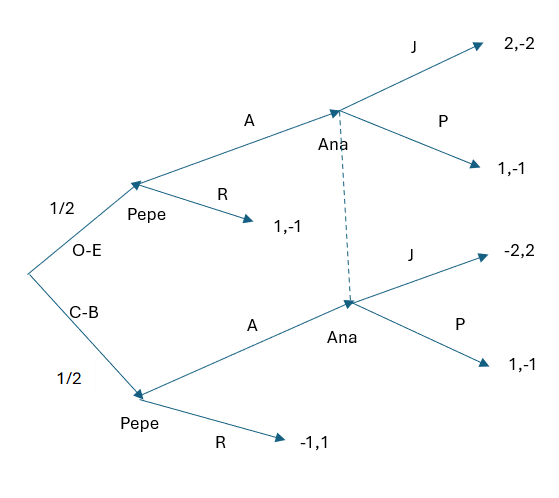
\includegraphics[width=0.8\linewidth]{forma_extensiva} 

}

\caption{\label{forma_extensiva}Diagrama Juego en Forma Extensiva}\label{fig:forma_extensiva}
\end{figure}

La linea discontinua uniendo los dos nodos donde participa la jugadora
Ana denotan que no sabe en que parte del árbol se encuentra, es decir,
hace si apuesta o se retira sin saber de que palo es la carta que saca

Al igual que hicimos en la forma normal de un juego, vamos a
caracterizar la forma extensiva de un juego por los distintos elementos
que intervienen en tal representación

\emph{Definición} Un juego en forma extensiva \(\Gamma\) viene
caracterizado por una 7-tupla:
\[\Gamma=\{J,X,A,\{X_i\}_{i \in J},H,P,U \}\] Los elementos que lo
forman son:

*Conjunto de jugadores que participan en el juego \(J=\{1,\cdots,N\}\).
También es común denotar como jugador 0 a los movimientos que se
realizan aleatoriamente.

*\(X\), conjunto de nodos, que significan una posible situación del
juego. El nodo inicial se representa por \(o\). A partir de este
conjunto podemos diferenciar dos: \(T(X)\) conjunto de nodos terminales
del juego, y \(D(X)=X-T(X)\) los nodos donde algún jugador tiene que
tomar una decisión (no final)

*\(A\), conjunto de todas las posibles acciones del juego

*Para cada jugador \(i \in J\), sea \(X_i\) los nodos en los que el
jugador \(i\) tiene que tomar una decisión

*\(H\), familia de conjuntos de información que son la información que
conoce el jugador en cada nodo.

*Una función de probabilidad \[
\begin{array}{cccc}
P : & H_o \times A & \rightarrow & [0,1] \\
   &  (h,a) & \rightarrow   & P(h,a)
\end{array}
\] que proporciona una probabilidad a las acciones en los que interviene
el azar.

*Función de pagos o utilidad \[
\begin{array}{cccc}
U: & T(X) & \rightarrow & \mathbb{R}^N \\
   &  x & \rightarrow   & U(x)=(U_1(x),\cdots,U_N(x))
\end{array}
\] donde \(U_i(x)\) representa la utilidad que recibe el jugador i.
Podemos suponer que estas funciones son de Von Newmann-Morgenstern

Al igual que hicimos en el apartado anterior, vamos a formalizar el
ejemplo que hemos propuesto en forma extensiva: Tenemos los jugadores
\(J=\{0, Pepe, Ana\} = {0,1,2}\); el conjunto de nodos
\(X=\{0,x_1,x_2,x_3,x_4,x_5,x_6,x_7,x_7,x_8,x_9 \}\); el conjunto de
acciones \(A=\{Ac_1,Ac_2,Ac_3,Ac_4,Ac_5,Ac_6,Ac_7,Ac_8 \}\); los
conjuntos de decisión para cada jugador \(X_i, \ i \in J=\{0,1,2\}\),
\(X_0=\{o \}\), \(X_1=\{x_1,x_2 \}\), \(X_2= \{x_3,x_5 \}\) ; el
conjunto de información de la que disponen los jugadores
\(H=\{ \{o\}, \{x_1\},\{x_2\}, \{x_3,x_5\} \}\); la funcion de
probabilidad para cada una de las acciones en las que interviene el
azar, \(P(\{o\},a)=\frac{1}{2}\) y \(P(\{o\},b)=\frac{1}{2}\); y las
funciones de pagos que reciben los jugadores en los distintos nodos
finales, \(U(x_4)=(1,-1)\), \(U(x_6)=(-1,1)\), \(U(x_7)=(2,-2)\),
\(U(x_8)=(1,-1)\), \(U(x_9)=(-2,2)\), \(U(x_10)=(1,-1)\). Así pues,
vamos a ver el diagrama del juego con esta forma de escribirlo mas
rigurosa:

\begin{figure}[H]

{\centering 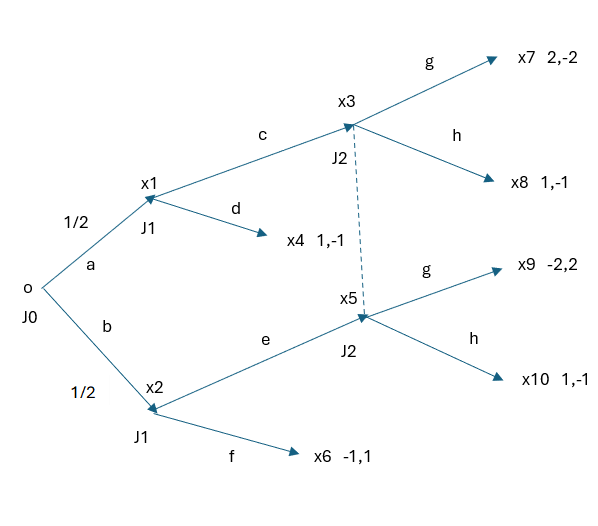
\includegraphics[width=0.8\linewidth]{forma_extensiva_rigurosa} 

}

\caption{\label{forma_extensiva_rigurosa}Diagrama Juego en Forma Extensiva Rigurosa}\label{fig:forma_extensiva_rigurosa}
\end{figure}

\hypertarget{Seccion23}{%
\section{Equilibrio de Nash}\label{Seccion23}}

De manera coloquial diríamos que un juego se encuentra en equilibrio si
ningún jugador obtiene mas utilidad al cambiar su estrategia de manera
unilateral, es decir, cada elección es la mejor respecto al resto de
elecciones de los adversarios, así ningún jugador tiene razones para
cambiar du elección y por tanto el juego se encuentra en equilibrio.
Pasamos a aportar una definición formal de este concepto.

\emph{Definición: Equilibrio de Nash en estrategias puras} Dado un juego
\(G=\{S_1,\cdots,S_n,U_1,\cdots,U_n\}\), un perfil de estrategias puras
\((s_1^*,\cdots,s_{i-1}^*,s_i^*,s_{i+1}^*,\cdots,s_n^*)\) es un
Equilibro de Nash si \[
\forall i \in N, \ U_i(s_1^*,\cdots,s_{i-1}^*,s_i^*,s_{i+1}^*,\cdots,s_n^*) \geq U_i(s_1^*,\cdots,s_{i-1}^*,s_i,s_{i+1}^*,\cdots,s_n^*), \ \forall s_i \ \text{de} \ S_i
\]

A continuación resolveremos los ejemplos que hemos seccionado en las
secciones \(\ref{Seccion221}\) y \(\ref{Seccion222}\)

\hypertarget{Seccion231}{%
\subsection{Resolución de un juego en forma normal}\label{Seccion231}}

Recordamos que tenemos el juego con la siguiente matriz: \[
\begin{array}{c|c|c}
 & \text{Montar} & \text{No Montar} \\
\hline
\text{Montar} & 1,1 & 4,0 \\
\hline
\text{No Montar} & 0,4 & 0,0 \\
\hline
\end{array}
\] En este juego tenemos las siguiente soluciones posibles:
(\(Montar\),\(Montar\)), (\(Montar\),\(No \ Montar\)),
(\(No \ Montar\),\(Montar\)) y (\(No \ Montar\),\(No \ Montar\)).

Comenzamos analizando la solución (\(No \ Montar\),\(No \ Montar\))
suponiendo que es un Equilibrio de Nash. Si la empresa A piensa que la
empresa B no montará el negocio es claro que no le interesa mantener su
decisión en no montar el negocio puesto que su utilidad aumenta de 0 a
4. De esta forma cualquiera de las dos empresas (ocurre lo mismo porque
son simétricas) cambiará su estrategia a montar el negocio.

Ahora analicemos el caso (\(Montar\),\(No \ Montar\)), que tiene un
razonamiento similar al caso (\(No \ Montar\),\(Montar\)), y volvemos a
suponer que es un Equilibrio de Nash. En esta situación, si la empresa B
supiese que la empresa A va a decidir montar el negocio esta cambiara su
estrategia y montaría también el negocio aumentando así su utilidad de 0
a 1. Por lo tanto estas dos opciones (\(Montar\),\(No \ Montar\)) y
(\(No \ Montar\),\(Montar\)) no son un equilibrio de Nash.

De esta forma solo nos quedaría la siguiente solución posible
(\(Montar\),\(Montar\)) que si es un Equilibrio de Nash puesto que ambas
empresas disminuyen la utilidad que perciben si alguna de ellas cambia a
no montar el negocio. De manera gráfica podemos representarlo con la
matriz anterior

\[
\begin{array}{c|c|c}
 & \text{Montar} & \text{No Montar} \\
\hline
\text{Montar} & \underline{1},\underline{1} & \underline{4},0 \\
\hline
\text{No Montar} & 0,\underline{4} & 0,0 \\
\hline
\end{array}
\] y (\(Montar\),\(Montar\)) es el equilibrio de Nash

\hypertarget{Seccion232}{%
\subsection{Resolución de un juego en forma
extensiva}\label{Seccion232}}

Recordemos que en la sección \(\ref{#Seccion222}\) llegado al siguiente
esquema del juego \(\ref{forma_extensiva_rigurosa}\)

En cuanto al jugador 2, este no sabe en cual de los nodos \(x_3\) o
\(x_5\) se encuentra pues no ve la carta que se saca de la baraja. Así,
se encuentra con una probabilidad de \(\frac{1}{2}\) de estar en \(x_3\)
o en \(x_5\). Si decidimos apostar, el valor esperado a ganar es
\(\frac{1}{2}*(-2) +\frac{1}{2}*2 =0\), mientras que si decide no
apostar y plantarse el valor esperado a ganar es
\(\frac{1}{2}*(-1) +\frac{1}{2}*(-1) =-1\), por lo que el jugador 2
decidirá apostar pues el valor esperado de la utilidad que recibe es
mayor en ese caso.

Por otra parte, el jugador 1 si sabe en cual de los nodos de decisión
\(x_1\) o \(x_2\) pues el si ve la carta que saca del mazo. De esta
forma si se encuentra en el nodo de decisión \(x_1\) puede decidir
plantarse y de esta forma se lleva con probabilidad 1 1 euro, mientras
que si decide apostar, como el jugador 2 siempre decide apostar (g),
tiene un valor esperado de utilidad de
\(\frac{1}{2}*(-2) +\frac{1}{2}*2 =0\) por lo que siempre decidirá
plantarse (d). Si se encuentra en \(x_2\), si decide plantarse (f) tiene
probabilidad 1 de perder 1 euro, mientras que si decide apostar, al
saber igual que antes que el jugador 2 siempre decide g, el valor
esperado de utilidad de \(\frac{1}{2}*2 +\frac{1}{2}*(-2) =0\) que es
mayor así que en este nodo siempre decide e.

\begin{figure}[H]

{\centering 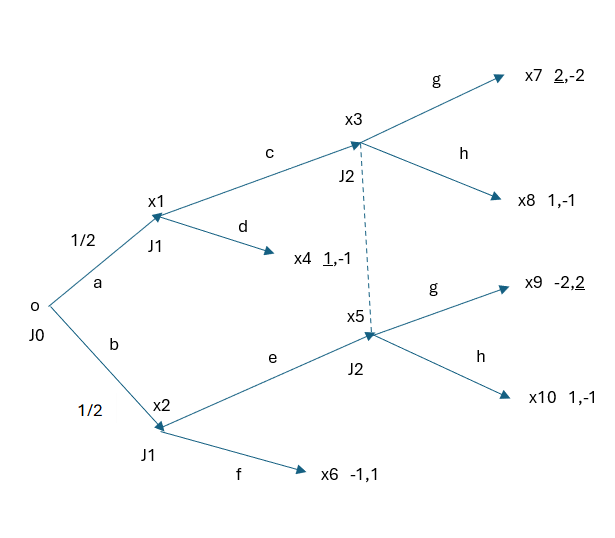
\includegraphics[width=0.8\linewidth]{forma_extensiva_equilibrio} 

}

\caption{\label{forma_extensiva_equilibrio}Diagrama Juego Forma Extensiva en Equilibrio}\label{fig:forma_extensiva_equilibrio}
\end{figure}

\FloatBarrier

\ifdefined\ifprincipal
\else
\setlength{\parindent}{1em}
\pagestyle{fancy}
\setcounter{tocdepth}{4}
\tableofcontents

\fi

\ifdefined\ifdoblecara
\fancyhead{}{}
\fancyhead[LE,RO]{\scriptsize\rightmark}
\fancyfoot[LO,RE]{\scriptsize\slshape \leftmark}
\fancyfoot[C]{}
\fancyfoot[LE,RO]{\footnotesize\thepage}
\else
\fancyhead{}{}
\fancyhead[RO]{\scriptsize\rightmark}
\fancyfoot[LO]{\scriptsize\slshape \leftmark}
\fancyfoot[C]{}
\fancyfoot[RO]{\footnotesize\thepage}
\fi

\renewcommand{\headrulewidth}{0.4pt}
\renewcommand{\footrulewidth}{0.4pt}

\hypertarget{Seccion3}{%
\chapter{Aplicación práctica: el blackjack}\label{Seccion3}}

\hypertarget{Seccion31}{%
\section{Cómo se juega al blacjack y qué tipo de juego
es}\label{Seccion31}}

El BlackJack, también conocido en lenguaje castellano como veintiuno, es
uno de los juegos mas populares en los casinos de todo el mundo junto
con el poker y la ruleta. A lo largo de estos últimos capítulos
buscaremos estudiar en profundidad este juego para encontrar la
estrategia optima con la que jugar para maximizar beneficios (o
minimizar pérdidas). La característica mas importante que convierte la
búsqueda de esta estrategia óptima en algo mas sencillo de lo que
pudiera parecer en un principio, es el hecho de que el crupier (persona
que reparte las cartas y asegura la normalidad del juego en cada mesa)
está obligado a jugar de manera fija y conocida por todos los jugadores.
Solo son los jugadores los que pueden ir tomando decisiones a lo largo
del juego siempre y cuando se sigan las reglas que ahora pasamos a
comentar.

\emph{Reglas del BlackJack}

\begin{itemize}
\item
  Usamos una baraje francesa de 52 cartas, es decir, 4 palos con 13
  cartas cada uno, del 1 al 10 y 3 figuras (las conocidas en España como
  sota, caballo y rey). Las cartas tienen unos valores: las figuras
  valen 10, y el resto de cartas tienen el mismo valor que su número,
  por ejemplo un 6 vale 6, menos el as que puede tomar los valores 1 u
  11 dependiendo de lo que prefiera el jugador (ya comentaremos en que
  situaciones preferirá que valga una cosa u otra.)
\item
  En el juego, a parte del crupier, participan como mucho 7 jugadores.
  Estos jugadores tienen que apostar el dinero antes de recibir la
  primera carta, lo que le da un atractivo al juego distinto al poker,
  en el que una vez recibamos cartas podemos aumentar la apuesta.
\item
  \textbf{Desempeño y estrategia del crupier.} En primer lugar, una vez
  todos los jugadores han hecho su apuestas, el crupier procede a
  repartir las cartas a los jugadores. Una vez que estos han hecho su
  juego, el crupier empieza a darse cartas a si mismo y está obligado a
  plantarse cuando la suma de las cartas que se haya dado sume al menos
  17. Cuando este tenga un as, que ya comentamos que pueden valer 1 u 11
  a gusto, deberá contarlo como 11 si al recibir el as y contarlo con
  valor 11 la suma de sus cartas es al menos 17. Para aclararlo, si
  tiene un 7 y la carta siguiente es un as, este contará como 11 puesto
  que la suma de los dos cartas sumarían 18, mientras que si por ejemplo
  tuviera un 3 y recibiera un as, no lo contará como 11 y su suma será
  4.
\item
  \textbf{Pagos.} Los pagos se basan en el hecho de ``ganar'' o no al
  crupier. Si el crupier se pasa y el jugador no lo hace, recibe una
  cantidad igual a su apuesta. Si no se pasan ninguno, quien mas se
  aproxime a 21 (de ahí el nombre del juego en español), si es el
  jugador recibe otra vez una cantidad igual a lo que ha apostado y si
  es el crupier se queda con el dinero apostado por el jugador. En caso
  de que empaten, no se producen juegos y el jugador recupera su dinero.
\item
  \textbf{BlackJack.} Esta jugada es la más famosa y la que da nombre al
  juego. Es la mano más poderosa y gana a cualquier otra mano que tenga
  el crupier. Si el jugador posee un blackjack y el crupier no, este
  último deberá pagarle al jugador el 150\% de su apuesta.
\item
  Otras posibilidades que tiene el jugador.

  \begin{itemize}
  \tightlist
  \item
    \textbf{Doblarse.} Si la suma de las dos primeras cartas es igual a
    9, 10 u 11, el jugador tiene la posibilidad de doblar su apuesta
    inicial, pero como desventaja solo podrá recibir una carta más.
  \item
    \textbf{Abrirse.} Cuando las dos primeras cartas que recibe el
    jugador tienen el mismo valor, un 10 y una figura o dos 7 por
    ejemplo, este puede separarlas y jugar a dos manos, teniendo que
    apostar en cada una la cantidad inicial que apostó. Si separamos un
    dos ases, al igual que pasaba antes cuando nos podíamos doblar, solo
    recibiremos una carta más en cada mano. Este apartado aunque parece
    ventajoso tiene el inconveniente de no poder abrirnos mas de una vez
    en cada jugada y en el caso de abrirnos con un as, en caso de
    recibir una carta que valga 10 puntos (figura o un 10) esto no
    contará como blackjack y en el caso de que el crupier lo obtuviese
    el jugador perdería el dinero de las dos manos.
  \item
    \textbf{Asegurarse.} En caso de que la primera carta que el crupier
    se reparta a si mismo sea un as, los jugadores tendrán la opción de
    asegurarse y prevenir un posible blackjack del crupier con una
    apuesta adicional de a lo mas el 50\% de la apuesta inicial. Si
    efectivamente ocurre que el crupier obtiene un blackjack, el jugador
    recibe por el seguro el doble de lo que apostó. Este seguro los
    jugadores deberán obtenerlo si así lo desean antes de que el crupier
    reparta la tercera carta al primer jugador que lo desee.
  \end{itemize}
\end{itemize}

\hypertarget{Seccion32}{%
\section{Estudio riguroso. Como jugar según la mano que
tengamos}\label{Seccion32}}

Llamemos \(x\) al valor total de las cartas que posee el jugador.
Consideramos dos tipos de manos que puede poseer un jugador: la que el
total del jugador es único y menor a 21, llamadas ``manos duras'', y la
que el jugador tiene uno o mas ases de manera que el jugador posee dos
cartas con valores menores a 21. A este último tipo de mano la
llamaremos ``manos blandas'' y requieren diferentes estudios a las manos
duras.

Definamos \(D\) como el valor de la carta mas alta que posee el crupier.
Así tomará los valores \(D=2, \cdots, 10, (1,11)\). Sea \(M(D)\) un
entero tal que si la carta mas alta del crupier es \(D\) y el valor
\(x\) es menor que \(M(D)\), el jugador debería pedir una carta más.
Mientras que dicho valor \(x\) sea al menos el valor de \(M(D)\), el
jugador deberá plantarse. De la misma manera definimos \(M^*(D)\) para
el caso de las manos blandas.

La suposición que hacemos es que una buena manera de saber cuando
dejamos de pedir cartas se da cuando tenemos al menos estos números
\(M(D)\) y \(M^*(D)\). Es decir, si hemos dicho que es bueno para
cualquier jugador dejar de pedir cartas si llegamos a ese valor, también
será correcto hacerlo cuando el valor de la mano sea incluso mayor. Esta
suposición suele ser correcta la mayoría de veces salvo en casos
especiales como cuando el hecho de dejar de pedir cartas se da cuando
los jugadores tienen manos bajas con un numero de cartas restantes a
repartir en el mazo bajo.

El primer paso es comparar la esperanza matemática de elegir \(M(D)=x\)
o \(M(D)=x+1\), con \(x\) tomando un valor único sin exceder 21. Para
las manos blandas comparamos \(M^*(D)=x\) con \(M^*(D)=x+1\). En ambos
casos empleamos la misma estrategia con la diferencia de que para el
primer caso una vez llegamos al valor nos paramos y para el otro pedimos
una carta mas. Para el caso de manos duras, comparar las dos esperanzas
es equivalente a comparar \(E_{p,x}\) la esperanza de pararse en un
total de \(x\), con \(E_{d,x}\), la esperanza de un jugador que con un
total de \(x\) pide una carta mas.Para el caso de las manos blandas, en
el primer caso el jugador se para mientras que en el otro pide una o más
cartas. Por ejemplo, en el caso de que tengamos una mano blanda con un
valor de 17 en el primer caso nos plantaríamos, mientras que en el
segundo caso pediríamos una carta mas. Pongamos que es un 5 por lo tanto
nos pasaríamos pero como el valor del as puede ser 1 u 11, seria de
valor 1 en este caso y obtenemos un total de 12, en cuyo caso deberíamos
pedir una carta mas en la mayoría de ocasiones.

A partir de ahora nos centramos en la diferencia de esas dos esperanzas
antes comentadas, \(E_{p,x}-E_{d,x}\) para ver si es mayor o menor que
0. Si fijamos un valor \(x\), la diferencia \(E_{p,x}-E_{d,x}\) es una
función decreciente en x, \(M(D)\) se obtiene como el menor valor de
\(x\) para el que \(E_{p,x}-E_{d,x} < 0\). Esta función es no creciente
siempre salvo casos excepcional como comentamos anteriormente en los que
crece con \(x\).

Definamos ahora \(T\) variable aleatoria como el valor final del
crupier. Sabemos por las reglas que comentamos en la apartado
\(\ref{Seccion31}\) que si ocurre que \(T>21\) o \(T<x\), el jugador
gana (en el caso de que se haya plantado con ese valor \(x\) en sus
cartas), mientras que si \(T=x\) cada uno recupera el dinero apostado, y
si \(x < T \leq 21\) el jugador pierde la apuesta. Así podemos definir
mejor la esperanza antes comentada:

\[
\begin{array}{ccl}
E_{p,x} & = & P(T>21) + P(T<x) - P(x<T \leq 21) \\
        & = & 2P(T>21) -1
\end{array}
\] Para el caso de la esperanza \(E_{d,x}\) definimos una nueva variable
aleatoria \(J\), que es la suma que le queda al jugador después de pedir
una carta mas (solo una). En caso de que el total pueda tener dos
valores sin exceder de 21 (caso de tener un as), \(J\) toma el mayor de
los dos valores.

Sabemos por las reglas que la mano del crupier siempre tiene un valor
mayor que 17 por lo que \(T \geq 17\), así que si \(J<17\), solo
ganaríamos en caso de que \(T>21\) y perderíamos para el resto de los
valores de la variable \(T\). Para este caso la esperanza sería:

\[
P(T>21) - P(T \leq 21)= 2P(T>21) -1
\]

Si el valor de las cartas del jugador es \(17 \leq J \leq 21\), la
esperanza quedaría como:

\[
P(T>21) +P(T<J) - P(J < T \leq 21)
\]

Lógicamente si el valor de la mano del jugador es \(J>21\) siempre vamos
a perder y por tanto esa esperanza sería -1, es decir perderíamos cada
euro apostado.

Una pregunta que podríamos hacernos es si estas variables \(T\) y \(J\)
son independientes. Analizando, El valor que tome la variable \(J\)
afecta a la variable \(T\) en solo si descartamos la posibilidad de que
el crupier desvele una carta de valor \(J-x\). Por lo tanto, si asumimos
la independencia de estas dos variables estaríamos cometiendo un pequeño
sesgo en el calculo de la esperanza. De esta manera:

\[
\begin{array}{ccl}
E_{d,x} & = & P(J<17)[2P(T>21)-1] - P(J>21) \\
        &   & + \Sigma_{j=17}^21 P(J=j) [P(T>21) + P(T<j) - P(j<T \leq21)]
\end{array}
\]

Ya tenemos calculadas las dos esperanzas. Restándolas nos queda:

\[
\begin{array}{ccl}
E_{d,x} -E_{p,x} & = & -2P(T<x) - P(T=x) -2P(T>21)P(J>21) \\
                 &   & + 2P(T<J \leq 21)+P(T=J \leq 21)
\end{array}
\]

Si \(T \geq 17\), los primeros dos términos son cero para el caso en que
\(x<17\). Además, \(P(J>21)\) es también cero para el caso de una mano
dura y menos de 12 para valores de una mano blanda. Por lo tanto esa
diferencia de esperanza \(E_{d,x} -E_{p,x} \geq 0\) para manos duras con
\(x<12\) y para manos blandas con \(x<17\), de lo que sacamos que
\(M(D)>11\) y \(M^*(D)>16\), \(\forall D\)

Consideremos ahora esta diferencia de esperanzas para el caso de valores
\(12 \leq x \geq 16\) en el caso de manos duras. Los dos primeros
términos vuelven a ser ceros, mientras que el ultimo lo podemos
reescribir usando la independencia entre \(J\) y \(T\) como usamos
anteriormente.

\[
E_{d,x} -E_{p,x} = -2P(T>21)P(J>21) + \sum_{t=17}^{21} P(T=t)[2P(t<J \leq 21) + P(J=t)]
\]

Ahora introducimos un supuesto, y es que la distribución de probabilidad
de \(J-x\), la única carta que pide el jugador está dada por:

\begin{itemize}
\item
  \(P(J-x=10) = 4/13\), del hecho de que tenemos 3 figuras más el 10 por
  cada palo en la baraja.
\item
  \(P(J-x=i) = 1/13, i=2,\cdots,9, (1,11)\)
\end{itemize}

De esta manera asumimos la suposición de que obtener una carta es
equiprobable. De primera mano podríamos danos cuenta de que esta
suposición es incorrecta en manos individuales, pero es cierta cuando
nos damos cuenta de que tenemos \(52!\) permutaciones posibles de cartas
en la baraja. Así pues, tendríamos lo siguiente:

\(P(J>21) = \frac{1}{13}(x-8)\), para \(x \geq 12\) en manos duras y
\(P(t<J \leq 21)=\frac{1}{13}(21-t)\), \(P(J=t) = \frac{1}{13}\) con
\(t\) tal que \(17 \leq t \leq 21\). Entonces:

\[
E_{d,x} - E_{p,x} = -2/13(x-8)P(T>21) + \sum_{t=17}^{21} 1/13(43-2t)P(T=t)
\]

Para valores de \(x\), \(12 \leq x \leq 16\) no necesitamos hacer esta
diferencia y ahora explicamos el porqué. Si la diferencia anterior la
igualamos a 0, y teniendo en cuenta que como comentamos la función es
decreciente en \(x\), se obtiene una única solución \(x_0\)

\[
x_0 = 8+ \frac{\sum_{t=17}^{21}(21 \frac{1}{2}-t)P(T=t)}{P(T>21)}
\] Así, si \(x_0 < 12\) entonces \(M(D)=12\). Si
\(x_0>16 entonces M(D)>16\) y si \(12 \leq x_0 \leq 16\) entonces
\(M(D) = [x_0]+1\) (parte entera de \(x_0\)). Para un valor dado de
\(P(T>17)\), mas probabilidad tiene el crupier de tener una buena mano,
mas bajo sea el numero en el que el jugador se pare. Por ejemplo, si
\(P(T>21)=2/5\) y \(P(T=18)=3/5\) entonces \(M(D)=14\) mientras que si
\(P(T>21)=2/5\) y \(P(T=19)=3/5\), entonces \(M(D)=12\).

En el caso de que \(x=17\) (en mano dura):

\[
E_{d,17}-E_{p,17} = -18/13P(T>21)- 5/13P(T=17)+ \sum_{t=18}^{21}1/13(43-2t)P(T=t)
\] Evaluando para cada \(t\) la probabilidad \(P(T=t)\) muestra que esa
diferencia en negativa para todo \(D\) y por tanto, \(M(D) \leq 17\).

Para el caso de manos blandas nos queda también el estudio cuando
\(x=17\). En esa situación,

\[
E_{d,17}-E_{p,17} = -1/13P(T=17)+ \sum_{t=18}^{21}1/13(43-2t)P(T=t)
\]

donde evaluando para cada \(t\) otra vez \(P(T=t)\), muestra que la
diferencia es positiva para todo \(D\) y por lo tanto \(M^*(D)>17\).

A partir de ahora, dado que siempre estamos comparando los estudios de
las manos duras con las manos blandas junto con los hechos de doblarse y
jugar a dos bandas, etc. Vamos a continuar el estudio por separado,
analizando bien cada situación para después sintetizar ambos resultados
en uno de carácter general.

\FloatBarrier

\ifdefined\ifprincipal
\else
\setlength{\parindent}{1em}
\pagestyle{fancy}
\setcounter{tocdepth}{4}
\tableofcontents

\fi

\ifdefined\ifdoblecara
\fancyhead{}{}
\fancyhead[LE,RO]{\scriptsize\rightmark}
\fancyfoot[LO,RE]{\scriptsize\slshape \leftmark}
\fancyfoot[C]{}
\fancyfoot[LE,RO]{\footnotesize\thepage}
\else
\fancyhead{}{}
\fancyhead[RO]{\scriptsize\rightmark}
\fancyfoot[LO]{\scriptsize\slshape \leftmark}
\fancyfoot[C]{}
\fancyfoot[RO]{\footnotesize\thepage}
\fi

\renewcommand{\headrulewidth}{0.4pt}
\renewcommand{\footrulewidth}{0.4pt}

\hypertarget{Seccion4}{%
\chapter{Estudios individuales en el BlackJack. Diferenciamos por
casos}\label{Seccion4}}

Hacemos un breve recordatorio de varios puntos que comentamos en el
apartado anterior y que vamos a utilizar individualmente en este
apartado

\textbf{Mano dura:} son aquellas manos del jugador que teniendo un as,
si este vale 11 podemos pasarnos de 21.

\textbf{Mano blanda:} son las manos del jugador que pueden tener un as
valiendo 11 sin excederse del total de 21. Si tomamos la decisión de
pedir una carta mas y con ella pasamos el límite, ese as pasa a tener
valor de 1.

\textbf{Suma de las cartas:} que notaremos por \(x\).

\textbf{Carta del crupier:} que notaremos por \(D\).

\textbf{Valor final del crupier:} que es una variable aleatoria notada
por \(T\).

\textbf{Suma del jugador:} es una variable aleatoria notada por \(J\)
que representa la suma del jugador tras pedir una única carta mas.

De aquí en adelante dejamos claro que la cantidad apostada por el
jugador es una unidad monetaria, ya sea euro o dolar, para asi
simplificar los calculos

\hypertarget{Seccion41}{%
\section{Manos duras}\label{Seccion41}}

Notemos por \(b\) la carta que se sirve el crupier.
\(b = 2, \cdots, 10, (1,11)\). Así pues en cada momento tenemos el para
\((x,b)\) en la que el jugador tiene la información de \(x\) puesto que
es el valor total de sus cartas y ve la carta que se sirve el crupier.
En esta situación el jugador debe decidir si parar y plantarse o pedir
mas cartas.

Definimos entonces \(G^*(x,b)\) como la máxima ganancia esperada por el
jugador dado una situación \((x,b)\) suponiendo que el jugador actúa de
forma optima y juega de manera racional.

De igual manera definimos \(G_0(x,b)\) como la ganancia esperada por el
jugador si este decide plantarse ante la situación del juego \((x,b)\).

Recordamos también que suponemos que la probabilidad de tener una
determinada carta de un valor es equiprobable es decir, la probabilidad
(notemos la como \(P_c\)) de obtener una carta de valor \(c\) es:

\[
P_c = 
\begin{cases}
4/13 & \text{si } c=10 \\
1/13 & \text{si } c \neq 10
\end{cases}
\] Con esta información podemos caracterizar \(G^*(x,b)\) como:

\[
G^*(x,b) = Max \\ \{G_0(x,b), \sum_{c=1}^{10}P_cG^*(x+c,b) \}
\]

Es decir, tenemos el máximo entre la opción de plantarnos en ese
instante o de la situación en la que nos encontraríamos si pidiéramos
una carta mas. Así nos plantaremos cuando el máximo lo alcancemos el
\(G_0(x,b)\).

Nos queda evaluar ese máximo para cada \(x\) y cada \(b\) posibles. Para
poder hacerlo necesitamos lo siguiente:

\begin{enumerate}
\def\labelenumi{\arabic{enumi}.}
\item
  \(G_0(x,b)\), \(\forall x=4, \cdots\) y
  \(\forall b= 2, \cdots, 10, (1,11)\)
\item
  Algunos valores finales de \(G^*(x,b)\) para iniciar el la inducción
  hacia atrás, \(\forall x,b\)
\end{enumerate}

\textbf{Calculo de \(G_0(x,b)\)}

De lo que obtuvimos en la sección anterior sabemos que:

\[ 
G_0(x,b) \ = \ Pr(T>21) \ + \ Pr(T<x) \ - \ Pr(x<T \leq 21) 
\] Ha de constar que esta ganancia se basa en que estamos apostando

Así pues el siguiente paso es calcular las probabilidades del crupier
que dada una carta de valor \(b\), la variable \(T\) tenga un
determinado valor final.

\textbf{Cálculo de las probabilidades de la variable \(T\) dada una
carta conocida \(b\)}

\begingroup\fontsize{12}{14}\selectfont

\begin{longtable}[t]{lccccccc}
\caption{\label{tab:unnamed-chunk-36}Probabilidades de resultado final del crupier según carta visible}\\
\toprule
 & 17 & 18 & 19 & 20 & 21 & BlackJack & Se pasa\\
\midrule
2 & 0.1377 & 0.1405 & 0.1320 & 0.1216 & 0.1140 & 0.0000 & 0.3542\\
3 & 0.1344 & 0.1349 & 0.1220 & 0.1260 & 0.1067 & 0.0000 & 0.3760\\
4 & 0.1360 & 0.1296 & 0.1135 & 0.1208 & 0.1106 & 0.0000 & 0.3895\\
5 & 0.1241 & 0.1201 & 0.1244 & 0.1107 & 0.1101 & 0.0000 & 0.4106\\
6 & 0.1646 & 0.1074 & 0.1071 & 0.1006 & 0.1006 & 0.0000 & 0.4197\\
\addlinespace
7 & 0.3718 & 0.1315 & 0.0775 & 0.0766 & 0.0761 & 0.0000 & 0.2665\\
8 & 0.1272 & 0.3651 & 0.1287 & 0.0688 & 0.0698 & 0.0000 & 0.2404\\
9 & 0.1168 & 0.1221 & 0.3481 & 0.1192 & 0.0630 & 0.0000 & 0.2308\\
Figura & 0.1133 & 0.1085 & 0.1164 & 0.3436 & 0.0328 & 0.0714 & 0.2140\\
As & 0.1296 & 0.1223 & 0.1260 & 0.1271 & 0.0544 & 0.3102 & 0.1304\\
\bottomrule
\end{longtable}
\endgroup{}

Ahí tenemos las probabilidades calculadas en función de cada carta
inicial que veamos. Si las comparamos con las de la biografía

\begin{figure}[H]

{\centering \includegraphics[width=0.8\linewidth]{tabla_probabilidades_español} 

}

\caption{\label{forma_extensiva}Diagrama Juego}\label{fig:español_blackjack}
\end{figure}

\begin{figure}[H]

{\centering 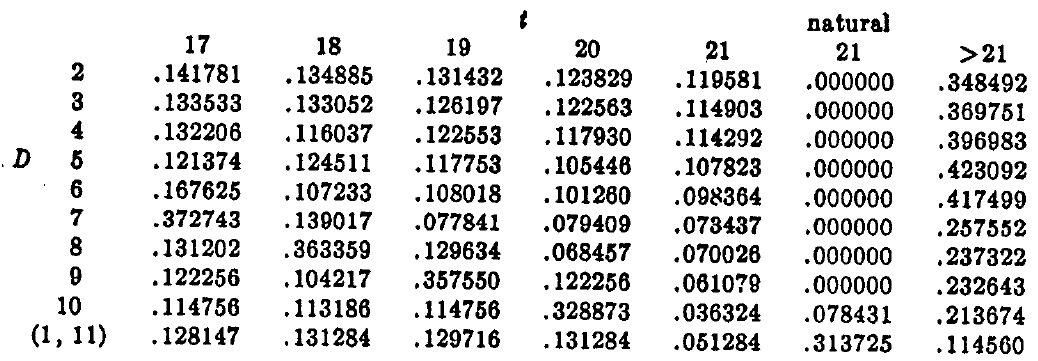
\includegraphics[width=0.8\linewidth]{tabla_probabilidades_baldwin} 

}

\caption{\label{forma_extensiva}Diagrama Juego}\label{fig:ingles_blackjack}
\end{figure}

Podemos ver que los resultados son muy similares, por lo que podemos
deducir que los cálculos que hemos realizado son correctos. Una vez
conocidas las probabilidades, ya estamos en disposición de calcular
\(G_0(x,b)\) como detallábamos al comienzo, \(\forall \ x=4,\cdots\) y
\(\forall \  b=2,\cdots,10,(1,11)\). Una vez construyamos los
\(G_0(x,b)\) los utilizamos para implementarlos en el algoritmo,
teniendo en cuenta que si el máximo lo alcanzamos en dicho valor nos
plantaremos, y en caso contrario pediremos carta.

\begingroup\fontsize{12}{14}\selectfont

\begin{longtable}[t]{lcccccccccc}
\caption{\label{tab:unnamed-chunk-38}Tabla de procedimientos si el jugador posee una mano dura}\\
\toprule
 & 2 & 3 & 4 & 5 & 6 & 7 & 8 & 9 & Figura & As\\
\midrule
4 & C & C & C & C & C & C & C & C & C & C\\
5 & C & C & C & C & C & C & C & C & C & C\\
6 & C & C & C & C & C & C & C & C & C & C\\
7 & C & C & C & C & C & C & C & C & C & C\\
8 & C & C & C & C & C & C & C & C & C & C\\
\addlinespace
9 & C & C & C & C & C & C & C & C & C & C\\
10 & C & C & C & C & C & C & C & C & C & C\\
11 & C & C & C & C & C & C & C & C & C & C\\
12 & C & C & C & C & C & C & C & C & C & C\\
13 & C & C & P & P & P & C & C & C & C & C\\
\addlinespace
14 & P & P & P & P & P & C & C & C & C & C\\
15 & P & P & P & P & P & C & C & C & C & C\\
16 & P & P & P & P & P & C & C & C & C & C\\
17 & P & P & P & P & P & P & P & P & P & P\\
18 & P & P & P & P & P & P & P & P & P & P\\
\addlinespace
19 & P & P & P & P & P & P & P & P & P & P\\
20 & P & P & P & P & P & P & P & P & P & P\\
21 & P & P & P & P & P & P & P & P & P & P\\
22 & P & P & P & P & P & P & P & P & P & P\\
23 & P & P & P & P & P & P & P & P & P & P\\
\addlinespace
24 & P & P & P & P & P & P & P & P & P & P\\
25 & P & P & P & P & P & P & P & P & P & P\\
26 & P & P & P & P & P & P & P & P & P & P\\
27 & P & P & P & P & P & P & P & P & P & P\\
28 & P & P & P & P & P & P & P & P & P & P\\
\addlinespace
29 & P & P & P & P & P & P & P & P & P & P\\
30 & P & P & P & P & P & P & P & P & P & P\\
31 & P & P & P & P & P & P & P & P & P & P\\
\bottomrule
\end{longtable}
\endgroup{}

\hypertarget{Seccion42}{%
\section{Manos blandas}\label{Seccion42}}

Ahora, nuestro propósito es hacer lo mismo para el caso de que el
jugador posea una mano blanda. La principal modificación reside en lo
que comentamos al comienzo, que si nos pasamos de 21 con este tipo de
manos recurrimos a contar ese As como un 1. Ahora llamamos
\(\bar G^*(x,b)\) a la ganancia esperada en el caso de manos blandas.

\[
\bar G^*(x,b) = Max \\ \{G_0(x,b), \sum_{c=1}^{10}P_c \bar G^*(x+c,b) \}
\] Como vemos la ecuación es exactamente igual al caso de manos duras.
Lo que diferencia el tratamiento son los valores finales que le damos a
\(\bar G^*(x,b)\), por el tratamiento diferente que reciben estas manos.
los valores iniciales son: \(\bar G^*(x,b) = G^*(x-10,b),x>21\) y
\(\forall b\)

Ahora nuestra regla de parada es la siguiente:

\begingroup\fontsize{12}{14}\selectfont

\begin{longtable}[t]{lcccccccccc}
\caption{\label{tab:unnamed-chunk-40}Tabla de procedimientos si el jugador posee una mano blanda}\\
\toprule
 & 2 & 3 & 4 & 5 & 6 & 7 & 8 & 9 & Figura & As\\
\midrule
4 & C & C & C & C & C & C & C & C & C & C\\
5 & C & C & C & C & C & C & C & C & C & C\\
6 & C & C & C & C & C & C & C & C & C & C\\
7 & C & C & C & C & C & C & C & C & C & C\\
8 & C & C & C & C & C & C & C & C & C & C\\
\addlinespace
9 & C & C & C & C & C & C & C & C & C & C\\
10 & C & C & C & C & C & C & C & C & C & C\\
11 & C & C & C & C & C & C & C & C & C & C\\
12 & C & C & C & C & C & C & C & C & C & C\\
13 & C & C & C & C & C & C & C & C & C & C\\
\addlinespace
14 & C & C & C & C & C & C & C & C & C & C\\
15 & C & C & C & C & C & C & C & C & C & C\\
16 & C & C & C & C & C & C & C & C & C & C\\
17 & C & C & C & C & C & C & C & C & C & C\\
18 & C & C & P & P & P & P & C & C & C & C\\
\addlinespace
19 & P & P & P & P & P & P & P & P & C & C\\
20 & P & P & P & P & P & P & P & P & P & C\\
21 & P & P & P & P & P & P & P & P & P & P\\
22 & P & P & P & P & P & P & P & P & P & P\\
23 & P & P & P & P & P & P & P & P & P & P\\
\addlinespace
24 & P & P & P & P & P & P & P & P & P & P\\
25 & P & P & P & P & P & P & P & P & P & P\\
26 & P & P & P & P & P & P & P & P & P & P\\
27 & P & P & P & P & P & P & P & P & P & P\\
28 & P & P & P & P & P & P & P & P & P & P\\
\addlinespace
29 & P & P & P & P & P & P & P & P & P & P\\
30 & P & P & P & P & P & P & P & P & P & P\\
31 & P & P & P & P & P & P & P & P & P & P\\
\bottomrule
\end{longtable}
\endgroup{}

\hypertarget{Seccion43}{%
\section{Doblar la apuesta}\label{Seccion43}}

Para poder doblarnos los valores de las dos primeras cartas deben sumar
9, 10 u 11, recibiendo una carta mas y solo una si lo hace. Así tenemos
las siguientes situaciones \((9,b)\), \((10,b)\), \((11,b)\),
\(\forall b\). Ahora tenemos que calcular la ganancia esperada de doblar
nuestra apuesta, en función de la carta que nos toque y compararla con
la ganancia esperada en el caso de no hacerlo, resultando en:

\[
\begin{array}{cllll}
\text{Si} & 2 \sum_{c=1}^{10}P_cG_0(x+c,b) & > & G^*(x,b) & \text{doblar apuesta} \\
\text{Si} & 2 \sum_{c=1}^{10}P_cG_0(x+c,b) & \leq & G^*(x,b) & \text{no doblar apuesta}\\
\end{array}
\]

Y la estrategia optima de cuando doblarse y cuando no es la siguiente:

\begingroup\fontsize{12}{14}\selectfont

\begin{longtable}[t]{lcccccccccc}
\caption{\label{tab:unnamed-chunk-42}Tabla de procedimientos para decidir si doblarse o no}\\
\toprule
 & 2 & 3 & 4 & 5 & 6 & 7 & 8 & 9 & Figura & As\\
\midrule
9 & D & D & D & D & D & No D & No D & No D & No D & No D\\
10 & D & D & D & D & D & D & D & D & No D & No D\\
11 & No D & No D & No D & No D & D & No D & No D & No D & No D & No D\\
\bottomrule
\end{longtable}
\endgroup{}

\hypertarget{Seccion44}{%
\section{Abrise y jugar a dos manos}\label{Seccion44}}

En este apartado tendremos que comparar la ganancia esperada cuando no
nos abrimos y jugamos de manera óptima como hicimos en los subapartados
\(\ref{#Seccion41}\) y \(\ref{#Seccion41}\), a la ganancia que
tendríamos en el caso de abrirnos y jugar óptimamente cada una de las
manos.

Así, construimos la siguiente regla que nos marca que camino tenemos que
coger:

\[
\begin{array}{cllll}
\text{Si} & 2 \sum_{c=1}^{10}P_cG^*(z+c,b) & > & G^*(2z,b) & \text{Abrirse} \\
\text{Si} & 2 \sum_{c=1}^{10}P_cG^*(z+c,b) & \leq & G^*(2z,b) & \text{No abrirse}\\
\end{array}
\] Donde \(z\) es la carta que recibimos doble. Aquí nos encontramos un
pequeño impedimento que es el caso cuando recibimos dos Ases, en este
caso tendríamos que:

\[
\begin{array}{cllll}
\text{Si} & 2 \sum_{c=1}^{10}P_cG_0(11+c,b) & > & \bar G^*(12,b) & \text{Abrirse} \\
\text{Si} & 2 \sum_{c=1}^{10}P_cG_0(11+c,b) & \leq & \bar G^*(12,b)& \text{No abrirse}\\
\end{array}
\]

Y obtendríamos las siguiente tabla con los procedimientos que debe
llevar el jugador:

\begingroup\fontsize{12}{14}\selectfont

\begin{longtable}[t]{lcccccccccc}
\caption{\label{tab:unnamed-chunk-44}Tabla de procedimientos para decidir si abrirse o no}\\
\toprule
 & 2 & 3 & 4 & 5 & 6 & 7 & 8 & 9 & Figura & As\\
\midrule
2-2 & No A & No A & No A & A & A & A & No A & No A & No A & No A\\
3-3 & No A & No A & No A & A & A & A & No A & No A & No A & No A\\
4-4 & No A & No A & No A & No A & No A & No A & No A & No A & No A & No A\\
5-5 & No A & No A & No A & No A & No A & No A & No A & No A & No A & No A\\
6-6 & No A & No A & A & A & A & No A & No A & No A & No A & No A\\
\addlinespace
7-7 & A & A & A & A & A & A & No A & No A & No A & No A\\
8-8 & A & A & A & A & A & A & A & A & No A & No A\\
9-9 & A & A & A & A & A & A & A & A & No A & No A\\
Figura-Figura & No A & No A & No A & No A & No A & No A & No A & No A & No A & No A\\
As-As & No A & A & A & A & A & No A & No A & No A & No A & No A\\
\bottomrule
\end{longtable}
\endgroup{}

\hypertarget{Seccion45}{%
\section{Asegurarse}\label{Seccion45}}

Suponemos ahora que la carta visible del crupier es un As. La apuesta
adicional que puede hacer el jugador es de un valor \(v\),
\(v \leq \frac{1}{2}\). Lo que ocurre aquí, es que el jugador decide
asegurarse, su mano ya no compite contra el crupier, sino que el compite
contra el hecho de que el crupier obtenga un BlacjJack. Por ejemplo, si
la suma de cartas del jugador es 13 y la primera carta del crupier es un
As, este podría asegurarse. En caso de hacerlo, si el crupier no
obtuviera BlackJack, obtuviera una suma de 20, el jugador gana aunque su
suma es inferior a la suma del crupier.

Esta apuesta por tanto se reduce al hecho de que salga una figura o no.
La probabilidad de que salga una figura, como desde un comienzo estamos
en la hipótesis de sucesos equiprobables, es de \(\frac{16}{52}\) que es
aproximadamente \(0.3077 \rightarrow 30,77 \%\). Llamemosle \(p\) a la
probabilidad de que salga una figura, obteniendo el crupier un
blackjack. Supongamos que la cantidad con la que nos aseguramos es
\(v=\frac{1}{2}\). Entonces nos interesa que el valor esperado al
asegurarnos sea no negativo al menos.

El valor esperado lo podemos calcular con la fórmula
\(E[ \ Asegurarse \ ]= 1·p - \frac{1}{2}·(1-p)\) veamos cuando esa
esperanza es mayor o igual a 0:

\[
\begin{array}{ccl}
p - \frac{1}{2}(1-p)& \geq  & 0 \\
p - \frac{1}{2} +\frac{1}{2}p& \geq  & 0\\
\frac{3}{2}p - \frac{1}{2} & \geq  & 0\\
3p - 1& \geq  & 0 \\
p & \geq & \frac{1}{3}
\end{array}
\] Es decir, para que asegurarse sea rentable la probabilidad debe ser
al menos de un tercio, \(33,3 \%\), por lo que no sería rentable
asegurarse, ya que la probabilidad que tenemos actualmente es inferior.
Esta probabilidad podría aumentar si el jugador viese si faltan muchas
figuras por salir de la baraja.

Como hemos asumido como hipótesis inicial que sacar una carta es
equiprobable a sacar otra, es decir, no contamos cartas, descartamos el
hecho de que asegurarse sea rentable a la larga y por lo tanto la
conclusion es no asegurarse.

Algo que podemos hacer es construir la forma normal del juego para ver
como sería este reparto:

\begingroup\fontsize{12}{14}\selectfont

\begin{longtable}[t]{lcc}
\caption{\label{tab:unnamed-chunk-45}Forma normal cuando jugador posee un Blackjack}\\
\toprule
 & C BJ & C No BJ\\
\midrule
J Asegura & 1 & 1.0\\
J No Asegura & 0 & 1.5\\
\bottomrule
\end{longtable}
\endgroup{}

Esto podríamos extenderlo a todos los casos, cuando la suma del jugador
es \(x\), que no es un Blackjack, y en caso de no conseguir un
Blackjack, la suma del crupier es \(T\) a lo siguiente y calcular las
ganancias esperadas en cada caso en función de la probabilidades de que
\(T\) supere a \(x\) o no

\hypertarget{Seccion46}{%
\section{Conclusion. Utilidad de seguir la estrategia
óptima.}\label{Seccion46}}

Ahora ya tenemos determinada nuestra estrategia optima, en la que
sabemos en que suma de cartas debemos plantando en función de si tenemos
una mano dura o una mano blanda; si debemos doblarnos o no dependiendo
de la carta que tenga visible el crupier; si debemos abrirnos y jugar a
dos manos siguiendo las estrategias anteriormente comentadas; y si
debemos asegurarnos, que sabemos que nunca lo debemos hacer.

Nuestro objetivo ahora es calcular cuantas unidades monetarias
obtendremos por cada una apostada en este juego, si siguiéramos la
estrategia ideal.

Para ello, para cada situación inicial que se presenta, carta visible
del crupier mas las dos cartas iniciales del jugador se genera una
cantidad grande de jugadas calculando la cantidad media de ganancia
obtenida en cada una mediante los métodos de montecarlo y se pondera por
la probabilidad de que suceda esa mano

\FloatBarrier

\ifdefined\ifprincipal
\else
\setlength{\parindent}{1em}
\pagestyle{fancy}
\setcounter{tocdepth}{4}
\tableofcontents

\fi

\ifdefined\ifdoblecara
\fancyhead{}{}
\fancyhead[LE,RO]{\scriptsize\rightmark}
\fancyfoot[LO,RE]{\scriptsize\slshape \leftmark}
\fancyfoot[C]{}
\fancyfoot[LE,RO]{\footnotesize\thepage}
\else
\fancyhead{}{}
\fancyhead[RO]{\scriptsize\rightmark}
\fancyfoot[LO]{\scriptsize\slshape \leftmark}
\fancyfoot[C]{}
\fancyfoot[RO]{\footnotesize\thepage}
\fi

\renewcommand{\headrulewidth}{0.4pt}
\renewcommand{\footrulewidth}{0.4pt}

\hypertarget{Seccion5}{%
\chapter{VNM-Póker y Khun-Póker}\label{Seccion5}}

En este último apartado comentaremos otro juego de azar que introdujeron
Von Newmann y Morgenstern, el VNM-Póker, junto con una variante que
amplía este juego y que se conoce como Khun-Poker. El primero fue
introducido en \emph{Theory of Games and Economic Behavior}, mientras
uqe el segundo se introdujo en \emph{A simplified two-person
poker.Contributions to the Theory of Games} .

Los dos juegos costan de dos jugadores, comunmente llamados ANN y Beth.
Cada una de ellas coge al azar una carta de la baraja sin enseñarsela a
la otra. Asi podriamos decir que los juegos presentan 4 parámetros:

\begin{enumerate}
\def\labelenumi{\arabic{enumi}.}
\item
  Hay una baraja con cartas de valores q van de 1 a \(S\).
\item
  Cada carta está representada \(r\) veces en la baraja.
\item
  Una apuesta inicial de \(m\) uds. monetarias q cada jugador realiza
  antes de empezar la partida.
\item
  Un valor final de la apuesta total de cada jugador, que denotamos como
  \(n\), al cual el jugador puede llegar añadiendo \(n-m\) uds.
  monetarias adicionales
\end{enumerate}

Como regla general se considera que \(m<n\).

\hypertarget{Seccion51}{%
\section{VNM-Póker. Explicación, estrategias y
equilibrios}\label{Seccion51}}

\textbf{\(VNM-Póker(S,r,m,n)\)} . El juego comienza repartiendo una
carta a cada jugador, y a continuación, Ann mueve primero y elige si
pasar, jugando así por m, o subir, jugando así por n.~Ahora nos
encontramos con dos posibles situaciones:

\begin{itemize}
\item
  Si Ann pasa, ambas jugadores revelan sus dos cartas, y el jugador que
  tenga la carta mas alta gana el bote, que como no se ha subido la
  apuesta es de \(2m\) uds. monetarias. Si hubiera empate, cada jugador
  recupera su dinero.
\item
  Si Ann elige subir, incrementa su apuesta hasta n.~Le toca el turno a
  Beth que tiene dos posibles movimientos, retirarse o seguir.
\end{itemize}

** Si Beth se retira, Ann se lleva el bote encima de la mesa que consta
de los \(n\) suyos mas los \(m\) de Beth, por lo que gana \(m\). La
carta de Beth no se levanta en este caso.

** Si Beth decide seguir la apuesta, ella también incrementa su apuesta
hasta \(n\). Entonces cada una revela su carta y el que tenga la carta
de mayor valor se lleva el bote completo de \(2n\) ganando así \(n\). De
la misma manera que antes, en caso de empate los jugadores recuperan su
dinero.

El juego podemos clasificarlo dentro de los de suma cero, puesto las
ganancias de uno viene de las perdidas del otro y al final el dinero que
se reparte es el dinero que proviene de las apuestas de los dos
jugadores. Procedemos ahora a representar la forma extensiva de este
juego.

\begin{figure}[H]

{\centering 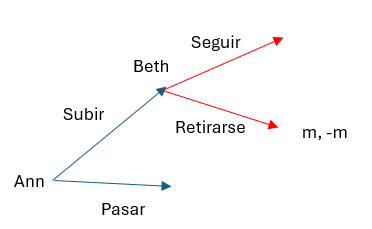
\includegraphics[width=0.8\linewidth]{extensiva_VNM} 

}

\caption{\label{forma_extensiva_VNM}VNM-Póker}\label{fig:VNM_Khun}
\end{figure}

Como hemos comentado, el juego comienza dándole una carta al azar a cada
jugador. Ann puede coger una carta cualquiera de \(1,\cdots,S\), y en
función del valor del parámetro \(r\) Beth podrá tomar también una carta
de \(1,\cdots,S\) dando \(S^2\) posibles combinaciones si \(r>1\) y en
caso de \(r = 1\), habría \(S(S-1)\) posibles combinaciones.

Con esto nos damos cuenta de que los parámetros intervienen de forma
distinta: mientras que \(m\) y \(n\) intervienen en el aspecto de
apuesta y reparto del dinero, los parámetros \(S\) y \(r\) tienen
influencia en la forma y tamaño del árbol del juego y las probabilidades
de los movimientos que dependen del azar.

Las alternativas para el movimiento aleatorio de recibir una determinada
carta no son igualmente probables. Por ejemplo, si fijamos una carta
determinada llamemosle \(C\), la probabilidad de obtener \(C\) es
\(\frac{r}{rS}= \frac{1}{S}\). una vez se saca dicha carta del mazo,
quedan \(r-1\) cartas \(C\) de un total de \(rS-1\), por lo que la
probabilidad de obtener otra carta \(C\) es \(\frac{r-1}{rS-1}\). Como
resumen:

\begin{itemize}
\tightlist
\item
  Si Ann y Beth tienen cartas de igual valor \(c\), esto tiene una
  probabilidad
\end{itemize}

\[
p_{cc}=\frac{1}{S} · \frac{r-1}{rS-1}=\frac{r-1}{S(rS-1)}
\]

\begin{itemize}
\tightlist
\item
  Si Ann y Beth tienen cartas de distinto valor \(c\) y \(d\), esto
  tiene una probabilidad
\end{itemize}

\[
p_{cd}=\frac{1}{S} · \frac{r}{rS-1}=\frac{r}{S(rS-1)}
\]

\emph{Ejemplo VNM-Póker(2,2,1,1)}

\begin{figure}[H]

{\centering 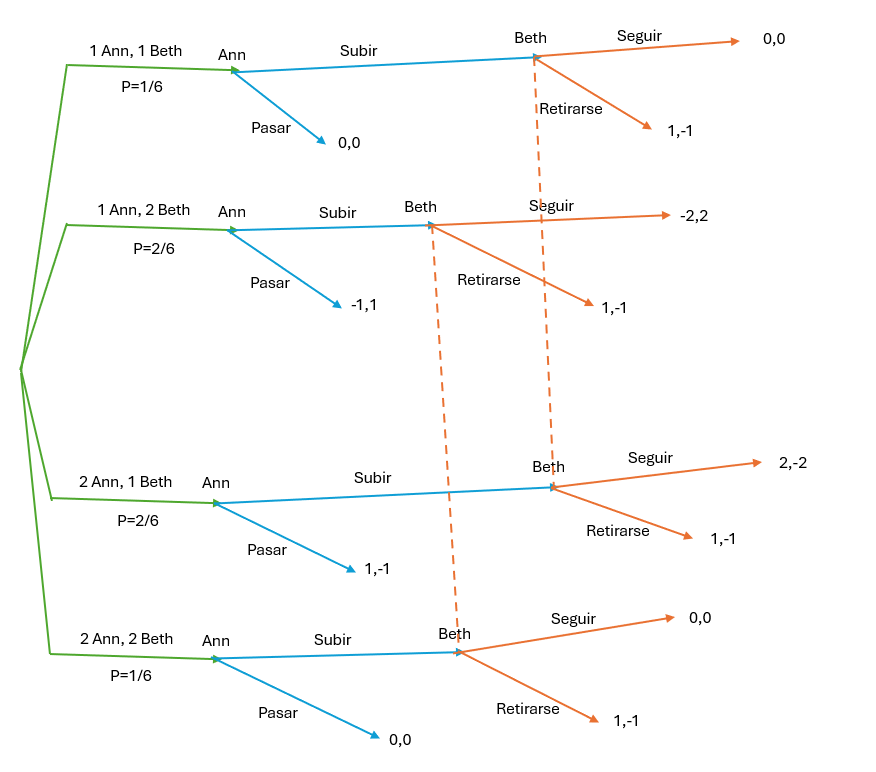
\includegraphics[width=0.8\linewidth]{Ejemplo_VNM} 

}

\caption{\label{ejemplo_VNM}VNM-Póker}\label{fig:ejemplo_VNM}
\end{figure}

\hypertarget{Seccion511}{%
\subsection{Estrategias}\label{Seccion511}}

Si \(r>1\) hay \(S*S\) diferentes combinaciones para repartir un valor a
Ann y otro a Beth. Ann como hemos dicho solo puede ver su carta por lo
que tiene \(S\) conjuntos de información. En cada uno de esos conjuntos
tiene las opciones de subir o pasar. Así pues, Ann tiene \(2^S\)
estrategias puras. Codificamos las estrategias por secuencias de \(R\) y
\(C\) (de check y raise, traducción de pasar y subir). Por ejemplo, para
\(S=4\) seria \(RCCR\) una posibilidad, que significa que Ann sube la
apuesta con las cartas mas alta y mas baja y pasa en las dos cartas
intermedias. De la misma manera, Beth tiene \(S\) conjuntos de
información con dos opciones y por lo tanto también tiene \(2^S\)
estrategias puras que están codificadas por \(C\) y \(F\) (traducciones
de seguir y retirarse).

De esta manera los posibles pagos son:

\begin{itemize}
\item
  Ann elige pasar \(\rightarrow\) \(m\), \(0\) ó \(-m\).
\item
  Ann elige subir y Beth elige retirarse \(\rightarrow\) \(m\).
\item
  Ann elige subir y Beth elige seguir \(\rightarrow\) \(n\), \(0\) ó
  \(n\).
\end{itemize}

En adelante supondremos \(S=2\) y \(r \geq 2\) . Suponiendo esto,
tenemos los siguientes conjuntos de estrategias puras para Ann es
\(\{CC \ (conservadora), CR \ (equilibrada),RC \ (inútil),RR \ (arriesgada) \}\)
y para Beth
\(\{FF \ (conservadora), FC \ (equilibrada),CF \ (inútil),CC \ (arriesgada) \}\)

Al igual que antes hicimos con la forma extensiva representamos la forma
normal del juego con \(S=2\)

\[
\begin{array}{c|c|c|c|c}
 & \text{FF} & \text{FC} & \text{CF} & \text{CC} \\
\hline
\text{CC} & 0 & 0 & 0 & 0 \\
\hline
\text{CR} & \frac{m(r-1)}{4r-2} & 0 & \frac{nr-m}{4r-2} & \frac{(n-m)r}{4r-2} \\
\hline
\text{RC} & \frac{m(3r-1)}{4r-2} & \frac{m(2r-1)-rn}{4r-2} & \frac{2mr}{4r-2} & \frac{r(m-n)}{4r-2}  \\
\hline
\text{RR} & m & \frac{m(2r-1)-rn}{4r-2} & \frac{m(2r-1)+rn}{4r-2} & 0 \\
\hline
\end{array}
\] Pasamos a comentar como hemos obtenido las expresiones para esta
tabla. Para cada par de estrategias, definimos \(u_{x,y}\) el pago que
recibe Ann cuando los jugadores siguen sus estrategias y Ann tiene una
carta de valor \(x\) y Beth una de valor \(y\), así la utilidad esperada
para Ann es la siguiente:

\[
p_{xx}u_{1,1} + p_{xy}u_{1,2} + p_{xy}u_{2,1} + p_{xx}u_{2,2}
\] donde \(p_{xx}=\frac{r-1}{4r-2}\) y \(p_{xy}=\frac{r}{4r-2}\)

Así, si Ann juega la estrategia \(RR\) y Beth juega \(FC\) tendríamos
las utilidades \(u_{1,1}=m\),\(u_{1,2}=-n\),\(u_{2,1}=m\) y\(u_{2,2}=0\)
y la utilidad que recibe Ann es:

\[
\begin{array}{ccl}
 &  & p_{xx}·m + p_{xx}·(-n) + p_{xx}·m + p_{xx}·0 \\
        & = & \frac{r-1}{4r-2}·m +\frac{r}{4r-2}·(-n) + \frac{r}{4r-2}·m +\frac{r-1}{4r-2}·0 \\
        & = & \frac{(r-1)m - rn +rm}{4r-2} \\
        & = & \frac{(2r-1)m-rn}{4r-2}·m
\end{array}
\]

Aunque hemos puesto en la tabla todas las estrategias posibles, somos
conscientes de que en algunos casos hay estrategias que están dominadas
por otras:

\begin{itemize}
\item
  Cuando Ann tiene una carta de mayor valor que Beth, subir domina a
  pasar.
\item
  Cuando Beth tiene una carta mas alta que la de Ann, seguir domina a
  retirarse.
\end{itemize}

Podemos extender esto a casos mas generales con el suiguiente teorema:

\textbf{Teorema}

Todas las estrategias de Beth, menos las de la forma \(C \cdots C\) y
las de la forma \(F \cdots FC \cdots C\) están debilmente dominadas.

Haciendo uso de este teorema podemos simplificar la forma normal del
juego a:

\[
\begin{array}{c|c|c|}
 & \text{FC} & \text{CC} \\
\hline
\text{CR} & 0  & \frac{(n-m)r}{4r-2} \\
\hline
\text{RR} & \frac{m(2r-1)-rn}{4r-2}  & 0 \\
\hline
\end{array}
\]

Una estrategia alternativa que podría seguir un jugador es la de
\emph{tirarse un farol} que consiste en, aun teniendo una carta de valor
bajo, este jugador decide subir la apuesta para intentando amedrentar al
otro jugador para así este decida retirarse. Desde el comienzo del
trabajo hemos supuesto la hipótesis de racionalidad de los jugadores por
lo que esta estrategia no tendría sentido. Pasemos ahora a analizar las
distintas estrategias.

\hypertarget{Seccion512}{%
\subsection{Análisis del juego}\label{Seccion512}}

\begin{itemize}
\tightlist
\item
  Equilibrio puro.
\end{itemize}

La entrada \(\frac{(n-m)r}{4r-2}\) siempre es \(>0\) puesto que \(n>m\).
Si \(\frac{(2r-1)m-rn}{4r-2}\) es \(<0\), la estrategia de Ann \(CR\)
domina débilmente a \(RR\), y la estrategia de Beth \(FC\) domina
débilmente a \(CC\). Por lo tanto, hay un equilibrio de Nash puro
\((CR,FC)\) con una utilidad esperada para Ann de \(0\).

\begin{itemize}
\tightlist
\item
  ¿Qué hacer si el adversario no juega de manera optima, sino mezclando
  estrategias puras no dominadas?
\end{itemize}

Vamos a suponer que el jugador que juega de esa manera es Beth, que lo
hace de esta manera: elige \(FC\) con una probabilidad \(q\) y elige
\(CC\) con probabilidad \(1-q\), es decir, elige seguir cuando tiene una
carta de valor 2 y retirarse con una probabilidad \(q\) cuando tiene una
carta de valor \(1\)

¿Qué tendría que hacer Ann en cada situación? Por un lado, si miramos
los pagos, Ann al jugar \(CR\) es \(\frac{(1-q)(n-m)r}{4r-2}\) que es
mayor o igual a \(\frac{q((2r-1)m-rn)}{4r-2}\) que es el pago al jugar
\(RR\) si (esto se da puesto que \(4r-2>0\) ya que \(r \geq 1\)):

\[
\begin{array}{rcl}
\frac{(1-q)(n-m)r}{4r-2} & \geq &\frac{q((2r-1)m-rn)}{4r-2}\\
(1-q)(n-m)r & \geq & q((2r-1)m-rn) \\
(n-m)r -q(n-m)r & \geq & q((2r-1)m-rn)\\
(n-m)r & \geq & q[((2r-1)m-rn)+(n-m)r]\\
(n-m)r & \geq & q[(r-1)m]\\
\end{array}
\]

Como \(r \geq 2\) tenemos que \((r-1)m >0\), lo podemos pasar dividiendo
sin cambiar el signo de la desigualdad y tendríamos:

\[
q^* = \frac{(n-m)r}{(r-1)m} \geq q
\] Por lo que Ann debe jugar \(CR\) si Beth juega \(FC\), mientras que
en otro caso Ann debería jugar \(RR\), jugando así de manera opuesta al
comportamiento de Beth. Por su parte, Beth debería copiar las jugadas
que haga Ann.

\begin{itemize}
\tightlist
\item
  Equilibrio mixto.
\end{itemize}

Si \(\frac{n}{m} \geq 2- \frac{1}{2}\) no hay equilibrio de Nash puro y
tendríamos q encontrar uno mixto.

Supongamos que Ann juega \(CR\) con probabilidad \(p\) y \(RR\) con
probabilidad \(1-p\), y Beth juega \(FC\) con probabilidad \(q\) y
\(CC\) con probabilidad \(1-q\). Cada una de las estrategias puras
\((CR,FC)\) y \((RR,CC)\) es una mejor respuesta a ellas y concluimos
con:

\[
p=\frac{(2r-1)m-rn}{(r-1)m} \ y \ q=\frac{(n-m)r}{(r-1)m}
\]

\hypertarget{Seccion52}{%
\section{Khun-Póker. Cambios respecto al VNM-Póker}\label{Seccion52}}

\textbf{\(Kuhn-Poker(S,r,m,n)\)} Este juego extiende el VNM-Póker. Si
Ann decide pasar los jugadores juegan un VNM-Póker con los roles
cambiados. Ann mueve primero eligiendo entre pasar o subir.

\begin{itemize}
\tightlist
\item
  Si Ann decide pasar, entonces Beth puede pasar o subir:
\end{itemize}

** Si Beth pasa, ambas cartas se levantan para ser visibles y el que
tenga la carta mas alta se lleva el bote, mientras que si empatan los
jugadores recuperan su dinero.

** Si Beth elige subir, incrementa su apuesta hasta \(n\). Entonces Ann
tiene dos opciones, retirarse o seguir.

*** Si Ann se retira, Beth se lleva la cantidad de \(n+m\), y la carta
de Ann no se revela.

*** Si Ann sigue, incrementa su apuesta hasta \(n\). Entonces ambas
cartas se revelan y el que tenga la carta mas alta se lleva los \(2n\)
de la apuesta y recuperan su dinero en caso de empate.

\begin{itemize}
\tightlist
\item
  Si Ann sube, el juego funciona como el VNM-Póker cuando Ann sube.
\end{itemize}

\begin{figure}[H]

{\centering 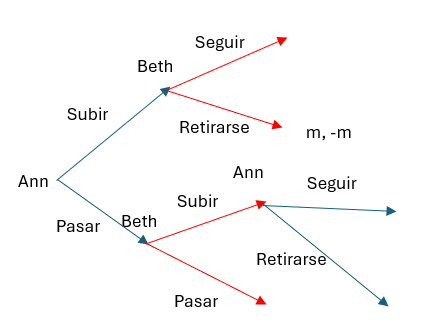
\includegraphics[width=0.8\linewidth]{extensiva_Kuhn} 

}

\caption{\label{forma_extensiva_VNM}Kuhn-Póker}\label{fig:forma_extensiva_VNM}
\end{figure}

\hypertarget{Seccion521}{%
\subsection{Estrategia}\label{Seccion521}}

Ann tiene \(2S\) conjuntos de información: o bien ella hace su primer
movimiento, subir o pasar, o Ann ha pasado en su primer movimiento, Beth
ha subido y entonces Ann puede seguir o retirarse. En todos eso casos,
ella solo conoce el valor de su carta. Beth tiene \(2S\) conjuntos de
información, determinados por el valor de su carta y en función de si
Ann ha subido o pasado, con \(S\) conjuntos de información en cada uno.

Por lo tanto, Ann tiene \(2^{2S}\) estrategias puras, indicadas por
\(S\) letras que pueden ser como en la sección \(\ref{Seccion511}\)
\(R\) o \(C\) para las elecciones de subir o pasar, y también \(S\)
letras \(F\) o \(C\) para la elección de retirarse o seguir. Así, para
\(S=2\) tenemos 16 estrategias puras, que son \(CCFF\), \(CCFC\),
\(CCCF\), \(CCCC\), \(CRFF\), \(CRFR\), \(CRCF\), \(CRCC\), \(RCFF\),
\(RCFC\), \(RCCF\), \(RCCC\), \(RRFF\),\(RRFC\), \(RRCF\), y \(RRCC\).

De la misma manera, Beth también tiene \(2S\) conjuntos de información,
\(S\) cuando Ann sube y otros \(S\) cuando Ann pasa, así para \(S=2\)
tendríamos: \(FFCC\), \(FFCR\), \(FFRC\), \(FFRR\), \(FCCC\), \(FCCR\),
\(FCRC\), \(FCRR\), \(CFCC\), \(CFCR\), \(CFRC\), \(CFRR\),
\(CCCC\),\(CCCR\), \(CCRC\), y \(CCRR\).

Hemos podido eliminar algunas estrategias por estar dominadas al igual
que antes. Si Ann tiene un valor de carta mayor que el de Beth, y ella
pasa cuando Beth sube, siempre es mejor para Ann seguir y no retirarse
puesto que retirándose pierde \(m\) uds. monetarias mientras que si
sigue no puede perder. Si Ann tiene un valor de carta mas alto, subir no
domina necesariamente a pasar, ya que depende de la estrategia de Beth.
Si Beth tiene una carta de valor mas alto que Ann, seguir domina a
retirarse y subir domina a pasar.

\FloatBarrier

\appendix

\ifdefined\ifprincipal
\else
\setlength{\parindent}{1em}
\pagestyle{fancy}
\setcounter{tocdepth}{4}
\tableofcontents

\fi

\ifdefined\ifdoblecara
\fancyhead{}{}
\fancyhead[LE,RO]{\scriptsize\rightmark}
\fancyfoot[LO,RE]{\scriptsize\slshape \leftmark}
\fancyfoot[C]{}
\fancyfoot[LE,RO]{\footnotesize\thepage}
\else
\fancyhead{}{}
\fancyhead[RO]{\scriptsize\rightmark}
\fancyfoot[LO]{\scriptsize\slshape \leftmark}
\fancyfoot[C]{}
\fancyfoot[RO]{\footnotesize\thepage}
\fi

\renewcommand{\headrulewidth}{0.4pt}
\renewcommand{\footrulewidth}{0.4pt}

\hypertarget{apuxe9ndice-tablas-de-ganancia-esperada}{%
\chapter{Apéndice: Tablas de ganancia
esperada}\label{apuxe9ndice-tablas-de-ganancia-esperada}}

\hypertarget{ganancias-esperadas-si-el-jugador-posee-una-mano-dura}{%
\section{Ganancias esperadas si el jugador posee una mano
dura}\label{ganancias-esperadas-si-el-jugador-posee-una-mano-dura}}

\begingroup\fontsize{12}{14}\selectfont

\begin{longtable}[t]{lcccccccccc}
\caption{\label{tab:unnamed-chunk-72}Tabla de ganancias si el jugador posee una mano dura}\\
\toprule
 & 2 & 3 & 4 & 5 & 6 & 7 & 8 & 9 & Figura & As\\
\midrule
4 & -0.106 & -0.067 & -0.050 & 0.001 & 0.016 & -0.057 & -0.129 & -0.205 & -0.306 & -0.414\\
5 & -0.120 & -0.080 & -0.062 & -0.010 & 0.004 & -0.087 & -0.156 & -0.230 & -0.328 & -0.432\\
6 & -0.132 & -0.092 & -0.073 & -0.021 & -0.007 & -0.118 & -0.185 & -0.255 & -0.350 & -0.451\\
7 & -0.103 & -0.063 & -0.045 & 0.004 & 0.030 & -0.060 & -0.191 & -0.254 & -0.342 & -0.462\\
8 & -0.027 & 0.010 & 0.026 & 0.069 & 0.107 & 0.080 & -0.066 & -0.198 & -0.287 & -0.399\\
\addlinespace
9 & 0.060 & 0.094 & 0.108 & 0.146 & 0.180 & 0.165 & 0.086 & -0.062 & -0.220 & -0.323\\
10 & 0.155 & 0.187 & 0.200 & 0.234 & 0.262 & 0.241 & 0.178 & 0.097 & -0.077 & -0.233\\
11 & 0.435 & 0.460 & 0.471 & 0.501 & 0.521 & 0.488 & 0.425 & 0.355 & 0.230 & 0.046\\
12 & -0.203 & -0.180 & -0.169 & -0.141 & -0.123 & -0.154 & -0.213 & -0.277 & -0.368 & -0.466\\
13 & -0.260 & -0.238 & -0.220 & -0.154 & -0.153 & -0.215 & -0.269 & -0.329 & -0.413 & -0.504\\
\addlinespace
14 & -0.296 & -0.244 & -0.220 & -0.154 & -0.153 & -0.271 & -0.321 & -0.377 & -0.455 & -0.540\\
15 & -0.296 & -0.244 & -0.220 & -0.154 & -0.153 & -0.323 & -0.370 & -0.421 & -0.494 & -0.572\\
16 & -0.296 & -0.244 & -0.220 & -0.154 & -0.153 & -0.371 & -0.415 & -0.463 & -0.530 & -0.603\\
17 & -0.152 & -0.105 & -0.086 & -0.036 & 0.015 & -0.104 & -0.380 & -0.408 & -0.460 & -0.602\\
18 & 0.126 & 0.161 & 0.174 & 0.202 & 0.286 & 0.397 & 0.107 & -0.171 & -0.235 & -0.347\\
\addlinespace
19 & 0.390 & 0.418 & 0.424 & 0.440 & 0.498 & 0.614 & 0.592 & 0.298 & -0.014 & -0.095\\
20 & 0.641 & 0.662 & 0.665 & 0.672 & 0.706 & 0.768 & 0.791 & 0.766 & 0.434 & 0.163\\
21 & 1.500 & 1.500 & 1.500 & 1.500 & 1.500 & 1.500 & 1.500 & 1.500 & 1.383 & 1.042\\
22 & -1.000 & -1.000 & -1.000 & -1.000 & -1.000 & -1.000 & -1.000 & -1.000 & -1.000 & -1.000\\
23 & -1.000 & -1.000 & -1.000 & -1.000 & -1.000 & -1.000 & -1.000 & -1.000 & -1.000 & -1.000\\
\addlinespace
24 & -1.000 & -1.000 & -1.000 & -1.000 & -1.000 & -1.000 & -1.000 & -1.000 & -1.000 & -1.000\\
25 & -1.000 & -1.000 & -1.000 & -1.000 & -1.000 & -1.000 & -1.000 & -1.000 & -1.000 & -1.000\\
26 & -1.000 & -1.000 & -1.000 & -1.000 & -1.000 & -1.000 & -1.000 & -1.000 & -1.000 & -1.000\\
27 & -1.000 & -1.000 & -1.000 & -1.000 & -1.000 & -1.000 & -1.000 & -1.000 & -1.000 & -1.000\\
28 & -1.000 & -1.000 & -1.000 & -1.000 & -1.000 & -1.000 & -1.000 & -1.000 & -1.000 & -1.000\\
\addlinespace
29 & -1.000 & -1.000 & -1.000 & -1.000 & -1.000 & -1.000 & -1.000 & -1.000 & -1.000 & -1.000\\
30 & -1.000 & -1.000 & -1.000 & -1.000 & -1.000 & -1.000 & -1.000 & -1.000 & -1.000 & -1.000\\
31 & -1.000 & -1.000 & -1.000 & -1.000 & -1.000 & -1.000 & -1.000 & -1.000 & -1.000 & -1.000\\
\bottomrule
\end{longtable}
\endgroup{}

\hypertarget{ganancias-esperadas-si-el-jugador-posee-una-mano-blanda}{%
\section{Ganancias esperadas si el jugador posee una mano
blanda}\label{ganancias-esperadas-si-el-jugador-posee-una-mano-blanda}}

\begingroup\fontsize{12}{14}\selectfont

\begin{longtable}[t]{lcccccccccc}
\caption{\label{tab:unnamed-chunk-74}Tabla de ganancias si el jugador posee una mano blanda}\\
\toprule
 & 2 & 3 & 4 & 5 & 6 & 7 & 8 & 9 & Figura & As\\
\midrule
4 & 0.44730 & 0.42799 & 0.41781 & 0.39345 & 0.40884 & 0.49892 & 0.52121 & 0.52921 & 0.52527 & 0.51830\\
5 & 0.44255 & 0.42220 & 0.41158 & 0.38590 & 0.40077 & 0.49740 & 0.52017 & 0.52928 & 0.52740 & 0.52271\\
6 & 0.43377 & 0.41256 & 0.40159 & 0.37466 & 0.38683 & 0.48632 & 0.51808 & 0.52761 & 0.52723 & 0.52685\\
7 & 0.40747 & 0.38561 & 0.37486 & 0.35049 & 0.36079 & 0.45200 & 0.49438 & 0.51348 & 0.51519 & 0.52191\\
8 & 0.37614 & 0.35639 & 0.34813 & 0.34078 & 0.37664 & 0.47438 & 0.45130 & 0.47716 & 0.48673 & 0.49712\\
\addlinespace
9 & 0.42498 & 0.42064 & 0.41591 & 0.40732 & 0.43786 & 0.53536 & 0.54189 & 0.46862 & 0.45207 & 0.45673\\
10 & 0.54237 & 0.53740 & 0.53256 & 0.52266 & 0.54649 & 0.62686 & 0.64262 & 0.63161 & 0.53124 & 0.43858\\
11 & 0.72454 & 0.71407 & 0.70832 & 0.69632 & 0.71029 & 0.77341 & 0.78621 & 0.78476 & 0.74020 & 0.63847\\
12 & 0.41324 & 0.39696 & 0.38836 & 0.36732 & 0.37612 & 0.44509 & 0.47334 & 0.49005 & 0.49899 & 0.50468\\
13 & 0.41708 & 0.39924 & 0.38803 & 0.35584 & 0.36748 & 0.44538 & 0.47428 & 0.49270 & 0.50499 & 0.51457\\
\addlinespace
14 & 0.41659 & 0.39007 & 0.37676 & 0.34233 & 0.35306 & 0.44821 & 0.47760 & 0.49740 & 0.51253 & 0.52545\\
15 & 0.40897 & 0.38075 & 0.36671 & 0.33011 & 0.34015 & 0.45429 & 0.48315 & 0.50417 & 0.52174 & 0.53719\\
16 & 0.39485 & 0.36523 & 0.35076 & 0.31326 & 0.32070 & 0.44838 & 0.48797 & 0.50822 & 0.52724 & 0.54901\\
17 & 0.33575 & 0.30686 & 0.29285 & 0.25484 & 0.23794 & 0.32563 & 0.45268 & 0.47963 & 0.49653 & 0.54016\\
18 & 0.21152 & 0.18114 & 0.17440 & 0.20180 & 0.28640 & 0.39650 & 0.24919 & 0.37923 & 0.42233 & 0.45954\\
\addlinespace
19 & 0.39040 & 0.41800 & 0.42380 & 0.44030 & 0.49850 & 0.61370 & 0.59230 & 0.29760 & 0.30470 & 0.37632\\
20 & 0.64060 & 0.66200 & 0.66540 & 0.67220 & 0.70600 & 0.76800 & 0.79090 & 0.76550 & 0.43360 & 0.16310\\
21 & 1.50000 & 1.50000 & 1.50000 & 1.50000 & 1.50000 & 1.50000 & 1.50000 & 1.50000 & 1.38270 & 1.04220\\
22 & -1.00000 & -1.00000 & -1.00000 & -1.00000 & -1.00000 & -1.00000 & -1.00000 & -1.00000 & -1.00000 & -1.00000\\
23 & -1.00000 & -1.00000 & -1.00000 & -1.00000 & -1.00000 & -1.00000 & -1.00000 & -1.00000 & -1.00000 & -1.00000\\
\addlinespace
24 & -1.00000 & -1.00000 & -1.00000 & -1.00000 & -1.00000 & -1.00000 & -1.00000 & -1.00000 & -1.00000 & -1.00000\\
25 & -1.00000 & -1.00000 & -1.00000 & -1.00000 & -1.00000 & -1.00000 & -1.00000 & -1.00000 & -1.00000 & -1.00000\\
26 & -1.00000 & -1.00000 & -1.00000 & -1.00000 & -1.00000 & -1.00000 & -1.00000 & -1.00000 & -1.00000 & -1.00000\\
27 & -1.00000 & -1.00000 & -1.00000 & -1.00000 & -1.00000 & -1.00000 & -1.00000 & -1.00000 & -1.00000 & -1.00000\\
28 & -1.00000 & -1.00000 & -1.00000 & -1.00000 & -1.00000 & -1.00000 & -1.00000 & -1.00000 & -1.00000 & -1.00000\\
\addlinespace
29 & -1.00000 & -1.00000 & -1.00000 & -1.00000 & -1.00000 & -1.00000 & -1.00000 & -1.00000 & -1.00000 & -1.00000\\
30 & -1.00000 & -1.00000 & -1.00000 & -1.00000 & -1.00000 & -1.00000 & -1.00000 & -1.00000 & -1.00000 & -1.00000\\
31 & -1.00000 & -1.00000 & -1.00000 & -1.00000 & -1.00000 & -1.00000 & -1.00000 & -1.00000 & -1.00000 & -1.00000\\
\bottomrule
\end{longtable}
\endgroup{}

\hypertarget{ganancias-esperadas-en-caso-de-doblarse-o-no-doblarse}{%
\section{Ganancias esperadas en caso de doblarse o no
doblarse}\label{ganancias-esperadas-en-caso-de-doblarse-o-no-doblarse}}

\begingroup\fontsize{12}{14}\selectfont

\begin{longtable}[t]{lcccccccccc}
\caption{\label{tab:unnamed-chunk-76}Tabla de ganancias al doblarse o no hacerlo}\\
\toprule
 & 2 & 3 & 4 & 5 & 6 & 7 & 8 & 9 & Figura & As\\
\midrule
9 & 0.06171 & 0.14245 & 0.17358 & 0.25738 & 0.32069 & 0.16484 & 0.08552 & -0.06189 & -0.21991 & -0.32305\\
10 & 0.35814 & 0.42923 & 0.45611 & 0.52545 & 0.57883 & 0.39674 & 0.28775 & 0.16725 & -0.07727 & -0.23306\\
11 & 0.43491 & 0.46048 & 0.47137 & 0.50149 & 0.53923 & 0.48777 & 0.42481 & 0.35504 & 0.23039 & 0.04640\\
\bottomrule
\end{longtable}
\endgroup{}

\hypertarget{ganancias-esperadas-en-caso-de-abrirse-o-no-abrirse}{%
\section{Ganancias esperadas en caso de abrirse o no
abrirse}\label{ganancias-esperadas-en-caso-de-abrirse-o-no-abrirse}}

\begingroup\fontsize{12}{14}\selectfont

\begin{longtable}[t]{lcccccccccc}
\caption{\label{tab:unnamed-chunk-78}Tabla de ganancias al abrirse o no hacerlo}\\
\toprule
 & 2 & 3 & 4 & 5 & 6 & 7 & 8 & 9 & Figura & As\\
\midrule
2-2 & -0.10610 & -0.06742 & -0.04959 & 0.03131 & 0.07186 & -0.02762 & -0.12885 & -0.20470 & -0.30578 & -0.41398\\
3-3 & -0.13224 & -0.09174 & -0.07313 & 0.00147 & 0.03234 & -0.08837 & -0.18453 & -0.25522 & -0.34978 & -0.45107\\
4-4 & -0.02695 & 0.01008 & 0.02623 & 0.06876 & 0.10687 & 0.08019 & -0.06555 & -0.19780 & -0.28666 & -0.39874\\
5-5 & 0.15465 & 0.18713 & 0.19965 & 0.23366 & 0.26230 & 0.24099 & 0.17846 & 0.09747 & -0.07727 & -0.23306\\
6-6 & -0.20330 & -0.17956 & -0.15246 & -0.04735 & -0.01660 & -0.15421 & -0.21268 & -0.27746 & -0.36807 & -0.46595\\
\addlinespace
7-7 & -0.18226 & -0.10265 & -0.06750 & 0.02786 & 0.08842 & -0.07044 & -0.32114 & -0.37699 & -0.45513 & -0.53952\\
8-8 & -0.00301 & 0.06997 & 0.10103 & 0.18274 & 0.26269 & 0.22943 & -0.05313 & -0.34029 & -0.53018 & -0.60295\\
9-9 & 0.19383 & 0.26164 & 0.28779 & 0.36028 & 0.42884 & 0.41076 & 0.26526 & -0.02101 & -0.23490 & -0.34670\\
Figura-Figura & 0.64060 & 0.66200 & 0.66540 & 0.67220 & 0.70600 & 0.76800 & 0.79090 & 0.76550 & 0.43360 & 0.16310\\
As-As & 0.41324 & 0.42923 & 0.45611 & 0.52545 & 0.57883 & 0.44509 & 0.47334 & 0.49005 & 0.49899 & 0.50468\\
\bottomrule
\end{longtable}
\endgroup{}

\ifdefined\ifprincipal
\else
\setlength{\parindent}{1em}
\pagestyle{fancy}
\setcounter{tocdepth}{4}
\tableofcontents

\fi

\ifdefined\ifdoblecara
\fancyhead{}{}
\fancyhead[LE,RO]{\scriptsize\rightmark}
\fancyfoot[LO,RE]{\scriptsize\slshape \leftmark}
\fancyfoot[C]{}
\fancyfoot[LE,RO]{\footnotesize\thepage}
\else
\fancyhead{}{}
\fancyhead[RO]{\scriptsize\rightmark}
\fancyfoot[LO]{\scriptsize\slshape \leftmark}
\fancyfoot[C]{}
\fancyfoot[RO]{\footnotesize\thepage}
\fi

\renewcommand{\headrulewidth}{0.4pt}
\renewcommand{\footrulewidth}{0.4pt}

\hypertarget{apuxe9ndice-codigo-r-utilizado-en-las-simulaciones}{%
\chapter{Apéndice: Codigo R utilizado en las
simulaciones}\label{apuxe9ndice-codigo-r-utilizado-en-las-simulaciones}}

\hypertarget{codigo-para-calcular-la-suma-final-del-crupier}{%
\section{Codigo para calcular la suma final del
crupier}\label{codigo-para-calcular-la-suma-final-del-crupier}}

\begin{Shaded}
\begin{Highlighting}[]
\FunctionTok{library}\NormalTok{(knitr)}
\FunctionTok{library}\NormalTok{(kableExtra)}
\FunctionTok{library}\NormalTok{(tidyverse)}
\NormalTok{Cartas }\OtherTok{\textless{}{-}} \FunctionTok{c}\NormalTok{(}\StringTok{"2"}\NormalTok{,}\StringTok{"3"}\NormalTok{,}\StringTok{"4"}\NormalTok{,}\StringTok{"5"}\NormalTok{,}\StringTok{"6"}\NormalTok{,}\StringTok{"7"}\NormalTok{,}\StringTok{"8"}\NormalTok{,}\StringTok{"9"}\NormalTok{,}\StringTok{"Figura"}\NormalTok{,}\StringTok{"As"}\NormalTok{)}
\NormalTok{Cantidad\_de\_cada\_carta }\OtherTok{\textless{}{-}} \FunctionTok{c}\NormalTok{(}\DecValTok{4}\NormalTok{,}\DecValTok{4}\NormalTok{,}\DecValTok{4}\NormalTok{,}\DecValTok{4}\NormalTok{,}\DecValTok{4}\NormalTok{,}\DecValTok{4}\NormalTok{,}\DecValTok{4}\NormalTok{,}\DecValTok{4}\NormalTok{,}\DecValTok{16}\NormalTok{,}\DecValTok{4}\NormalTok{)}
\NormalTok{Valor\_cartas }\OtherTok{\textless{}{-}} \FunctionTok{c}\NormalTok{(}\DecValTok{2}\NormalTok{,}\DecValTok{3}\NormalTok{,}\DecValTok{4}\NormalTok{,}\DecValTok{5}\NormalTok{,}\DecValTok{6}\NormalTok{,}\DecValTok{7}\NormalTok{,}\DecValTok{8}\NormalTok{,}\DecValTok{9}\NormalTok{,}\DecValTok{10}\NormalTok{,}\DecValTok{11}\NormalTok{)}
\NormalTok{Probabilidades\_sacar\_carta }\OtherTok{=}\NormalTok{ Cantidad\_de\_cada\_carta}\SpecialCharTok{/}\FunctionTok{sum}\NormalTok{(Cantidad\_de\_cada\_carta)}
\NormalTok{Valor\_cartas\_mano\_dura }\OtherTok{=}\FunctionTok{c}\NormalTok{(}\DecValTok{2}\NormalTok{,}\DecValTok{3}\NormalTok{,}\DecValTok{4}\NormalTok{,}\DecValTok{5}\NormalTok{,}\DecValTok{6}\NormalTok{,}\DecValTok{7}\NormalTok{,}\DecValTok{8}\NormalTok{,}\DecValTok{9}\NormalTok{,}\DecValTok{10}\NormalTok{,}\DecValTok{1}\NormalTok{)}
\NormalTok{Valor\_cartas\_mano\_blanda }\OtherTok{=}\NormalTok{ Valor\_cartas}

\NormalTok{encuentra\_as\_en\_mano }\OtherTok{\textless{}{-}} \ControlFlowTok{function}\NormalTok{(mano)\{}
  \ControlFlowTok{if}\NormalTok{ (}\StringTok{"As"} \SpecialCharTok{\%in\%}\NormalTok{ mano) \{}
    \FunctionTok{return}\NormalTok{(}\ConstantTok{TRUE}\NormalTok{)}
\NormalTok{  \} }\ControlFlowTok{else}\NormalTok{ \{}
    \FunctionTok{return}\NormalTok{(}\ConstantTok{FALSE}\NormalTok{)}
\NormalTok{  \}}
\NormalTok{\}}

\NormalTok{cuenta\_ases\_mano }\OtherTok{\textless{}{-}} \ControlFlowTok{function}\NormalTok{(mano)\{}
\NormalTok{  numero\_ases}\OtherTok{=}\DecValTok{0}
  \ControlFlowTok{for}\NormalTok{ (carta }\ControlFlowTok{in}\NormalTok{ mano) \{}
    \ControlFlowTok{if}\NormalTok{ (carta}\SpecialCharTok{==}\StringTok{"As"}\NormalTok{) \{}
\NormalTok{      numero\_ases}\OtherTok{=}\NormalTok{numero\_ases}\SpecialCharTok{+}\DecValTok{1}
\NormalTok{    \}}
\NormalTok{  \}}
  \FunctionTok{return}\NormalTok{(numero\_ases)}
\NormalTok{\}}


\NormalTok{Devuelve\_salida }\OtherTok{\textless{}{-}} \ControlFlowTok{function}\NormalTok{(suma,mano)\{}
  \ControlFlowTok{if}\NormalTok{ ((}\FunctionTok{all}\NormalTok{(}\FunctionTok{sort}\NormalTok{(mano) }\SpecialCharTok{==} \FunctionTok{sort}\NormalTok{(}\FunctionTok{c}\NormalTok{(}\StringTok{"Figura"}\NormalTok{, }\StringTok{"As"}\NormalTok{))))) \{}
    \FunctionTok{return}\NormalTok{(}\StringTok{"BlackJack"}\NormalTok{)}
\NormalTok{  \} }\ControlFlowTok{else}\NormalTok{\{}
    \ControlFlowTok{if}\NormalTok{ (suma }\SpecialCharTok{\textgreater{}}\DecValTok{21}\NormalTok{) \{}
      \FunctionTok{return}\NormalTok{(}\StringTok{"Se pasa"}\NormalTok{)}
\NormalTok{    \} }\ControlFlowTok{else}\NormalTok{\{}
      \FunctionTok{return}\NormalTok{(}\FunctionTok{as.character}\NormalTok{(suma))}
\NormalTok{    \}}
\NormalTok{  \} }
\NormalTok{\} }


\NormalTok{Calcular\_suma\_mano\_crupier }\OtherTok{\textless{}{-}} \ControlFlowTok{function}\NormalTok{(mano)\{}
\NormalTok{  suma}\OtherTok{=}\DecValTok{0}
  \ControlFlowTok{if}\NormalTok{ ((}\FunctionTok{all}\NormalTok{(}\FunctionTok{sort}\NormalTok{(mano) }\SpecialCharTok{==} \FunctionTok{sort}\NormalTok{(}\FunctionTok{c}\NormalTok{(}\StringTok{"Figura"}\NormalTok{, }\StringTok{"As"}\NormalTok{))))) \{}
\NormalTok{    suma }\OtherTok{=} \DecValTok{21}
\NormalTok{  \} }\ControlFlowTok{else}\NormalTok{ \{}
    \ControlFlowTok{if}\NormalTok{ (}\FunctionTok{encuentra\_as\_en\_mano}\NormalTok{(mano)) \{}
\NormalTok{      mano\_sin\_ases }\OtherTok{\textless{}{-}}\NormalTok{ mano[mano }\SpecialCharTok{!=} \StringTok{"As"}\NormalTok{]}
\NormalTok{      mano\_solo\_ases }\OtherTok{\textless{}{-}}\NormalTok{ mano[mano }\SpecialCharTok{==} \StringTok{"As"}\NormalTok{]}
      \ControlFlowTok{for}\NormalTok{ (carta }\ControlFlowTok{in}\NormalTok{ mano\_sin\_ases) \{}
\NormalTok{        suma}\OtherTok{=}\NormalTok{ suma }\SpecialCharTok{+}\NormalTok{ Valor\_cartas[}\FunctionTok{which}\NormalTok{(Cartas }\SpecialCharTok{==}\NormalTok{ carta)]}
\NormalTok{      \}}
      \ControlFlowTok{while}\NormalTok{ (}\FunctionTok{cuenta\_ases\_mano}\NormalTok{(mano\_solo\_ases)}\SpecialCharTok{\textgreater{}}\DecValTok{0}\NormalTok{) \{}
        \ControlFlowTok{if}\NormalTok{ ((suma }\SpecialCharTok{+} \DecValTok{11}\SpecialCharTok{\textgreater{}=}\DecValTok{17}\NormalTok{) }\SpecialCharTok{\&\&}\NormalTok{ (suma }\SpecialCharTok{+} \DecValTok{11} \SpecialCharTok{\textless{}=} \DecValTok{21}\NormalTok{)) \{}
\NormalTok{          suma }\OtherTok{=}\NormalTok{ suma}\SpecialCharTok{+}\DecValTok{11}
\NormalTok{        \} }\ControlFlowTok{else}\NormalTok{\{}
\NormalTok{          suma}\OtherTok{=}\NormalTok{suma}\SpecialCharTok{+}\DecValTok{1}\NormalTok{\}}
\NormalTok{        mano\_solo\_ases }\OtherTok{=}\NormalTok{mano\_solo\_ases[}\SpecialCharTok{{-}}\DecValTok{1}\NormalTok{]}
\NormalTok{      \}}
\NormalTok{    \} }
    \ControlFlowTok{else}\NormalTok{ \{}
      \ControlFlowTok{for}\NormalTok{ (carta }\ControlFlowTok{in}\NormalTok{ mano) \{}
\NormalTok{        suma}\OtherTok{=}\NormalTok{ suma }\SpecialCharTok{+}\NormalTok{ Valor\_cartas[}\FunctionTok{which}\NormalTok{(Cartas }\SpecialCharTok{==}\NormalTok{ carta)]}
\NormalTok{      \}}
\NormalTok{    \}}
\NormalTok{  \}}
  \FunctionTok{return}\NormalTok{(suma)}
\NormalTok{\}}

\NormalTok{Mano\_dada\_crupier }\OtherTok{\textless{}{-}} \ControlFlowTok{function}\NormalTok{(b)\{ }\CommentTok{\#b es la carta que todos ven que tiene el crupier}
\NormalTok{  suma}\OtherTok{=}\DecValTok{0}
\NormalTok{  mano}\OtherTok{=}\FunctionTok{c}\NormalTok{(b)}
  \ControlFlowTok{while}\NormalTok{ (suma}\SpecialCharTok{\textless{}}\DecValTok{17}\NormalTok{) \{}
\NormalTok{    carta\_1 }\OtherTok{\textless{}{-}} \FunctionTok{sample}\NormalTok{(Cartas,}\AttributeTok{size =} \DecValTok{1}\NormalTok{,}\AttributeTok{prob =}\NormalTok{ Probabilidades\_sacar\_carta)  }
\NormalTok{    mano }\OtherTok{=} \FunctionTok{c}\NormalTok{(mano,carta\_1)}
\NormalTok{    suma}\OtherTok{=}\FunctionTok{Calcular\_suma\_mano\_crupier}\NormalTok{(mano)}
\NormalTok{  \}}
  \FunctionTok{Devuelve\_salida}\NormalTok{(suma,mano)}
\NormalTok{\}}

\NormalTok{resultados\_tabla }\OtherTok{\textless{}{-}} \FunctionTok{data.frame}\NormalTok{()}

\CommentTok{\# Calcular probabilidades para cada carta visible}
\ControlFlowTok{for}\NormalTok{ (carta }\ControlFlowTok{in}\NormalTok{ Cartas) \{}
\NormalTok{  salida }\OtherTok{\textless{}{-}} \FunctionTok{replicate}\NormalTok{(}\DecValTok{10000}\NormalTok{, }\FunctionTok{Mano\_dada\_crupier}\NormalTok{(carta))}
\NormalTok{  tabla }\OtherTok{\textless{}{-}} \FunctionTok{prop.table}\NormalTok{(}\FunctionTok{table}\NormalTok{(}\FunctionTok{factor}\NormalTok{(salida, }
                                   \AttributeTok{levels =} \FunctionTok{c}\NormalTok{(}\StringTok{"17"}\NormalTok{,}\StringTok{"18"}\NormalTok{,}\StringTok{"19"}\NormalTok{,}\StringTok{"20"}\NormalTok{,}\StringTok{"21"}\NormalTok{,}\StringTok{"BlackJack"}\NormalTok{,}\StringTok{"Se pasa"}\NormalTok{))))}
\NormalTok{  resultados\_tabla }\OtherTok{\textless{}{-}} \FunctionTok{rbind}\NormalTok{(resultados\_tabla, }\FunctionTok{as.numeric}\NormalTok{(tabla))}
  \FunctionTok{colnames}\NormalTok{(resultados\_tabla)}\OtherTok{=}\FunctionTok{c}\NormalTok{(}\StringTok{"17"}\NormalTok{,}\StringTok{"18"}\NormalTok{,}\StringTok{"19"}\NormalTok{,}\StringTok{"20"}\NormalTok{,}\StringTok{"21"}\NormalTok{,}\StringTok{"BlackJack"}\NormalTok{,}\StringTok{"Se pasa"}\NormalTok{)}
\NormalTok{\}}
\FunctionTok{rownames}\NormalTok{(resultados\_tabla)}\OtherTok{=}\FunctionTok{c}\NormalTok{(}\StringTok{"2"}\NormalTok{,}\StringTok{"3"}\NormalTok{,}\StringTok{"4"}\NormalTok{,}\StringTok{"5"}\NormalTok{,}\StringTok{"6"}\NormalTok{,}\StringTok{"7"}\NormalTok{,}\StringTok{"8"}\NormalTok{,}\StringTok{"9"}\NormalTok{,}\StringTok{"Figura"}\NormalTok{,}\StringTok{"As"}\NormalTok{)}


\NormalTok{Calculo\_G\_0 }\OtherTok{\textless{}{-}} \ControlFlowTok{function}\NormalTok{(x, b, tabla, }\AttributeTok{es\_blackjack =} \ConstantTok{FALSE}\NormalTok{) \{}
\NormalTok{  probabilidades\_final\_crupier }\OtherTok{\textless{}{-}}\NormalTok{ tabla[b, ]}
  
  \CommentTok{\# Extraemos probabilidades}
\NormalTok{  pr\_T\_17\_20 }\OtherTok{\textless{}{-}} \FunctionTok{as.numeric}\NormalTok{(probabilidades\_final\_crupier[}\FunctionTok{c}\NormalTok{(}\StringTok{"17"}\NormalTok{, }\StringTok{"18"}\NormalTok{, }\StringTok{"19"}\NormalTok{, }\StringTok{"20"}\NormalTok{)])}
\NormalTok{  pr\_T\_21 }\OtherTok{\textless{}{-}}\NormalTok{ probabilidades\_final\_crupier}\SpecialCharTok{$}\StringTok{"21"}
\NormalTok{  pr\_T\_bj }\OtherTok{\textless{}{-}}\NormalTok{ probabilidades\_final\_crupier}\SpecialCharTok{$}\StringTok{"BlackJack"}
\NormalTok{  pr\_T\_pasa }\OtherTok{\textless{}{-}}\NormalTok{ probabilidades\_final\_crupier}\SpecialCharTok{$}\StringTok{\textasciigrave{}}\AttributeTok{Se pasa}\StringTok{\textasciigrave{}}
  
  \ControlFlowTok{if}\NormalTok{ (x }\SpecialCharTok{\textgreater{}} \DecValTok{21}\NormalTok{) \{}
    \FunctionTok{return}\NormalTok{(}\SpecialCharTok{{-}}\DecValTok{1}\NormalTok{)}
\NormalTok{  \}}
  
  \ControlFlowTok{if}\NormalTok{ (x }\SpecialCharTok{==} \DecValTok{21} \SpecialCharTok{\&\&}\NormalTok{ es\_blackjack) \{}
    \FunctionTok{return}\NormalTok{(}\FloatTok{1.5} \SpecialCharTok{*}\NormalTok{ (}\DecValTok{1} \SpecialCharTok{{-}}\NormalTok{ pr\_T\_bj))  }\CommentTok{\# 0 * pr\_T\_bj es innecesario}
\NormalTok{  \}}
  
\NormalTok{  pr\_T\_menor }\OtherTok{\textless{}{-}} \FunctionTok{sum}\NormalTok{(pr\_T\_17\_20[}\FunctionTok{which}\NormalTok{(}\DecValTok{17}\SpecialCharTok{:}\DecValTok{20} \SpecialCharTok{\textless{}}\NormalTok{ x)])}
\NormalTok{  pr\_T\_igual }\OtherTok{\textless{}{-}} \FunctionTok{sum}\NormalTok{(pr\_T\_17\_20[}\FunctionTok{which}\NormalTok{(}\DecValTok{17}\SpecialCharTok{:}\DecValTok{20} \SpecialCharTok{==}\NormalTok{ x)]) }\SpecialCharTok{+} \FunctionTok{ifelse}\NormalTok{(x }\SpecialCharTok{==} \DecValTok{21}\NormalTok{, pr\_T\_21, }\DecValTok{0}\NormalTok{)}
\NormalTok{  pr\_T\_mayor }\OtherTok{\textless{}{-}} \FunctionTok{sum}\NormalTok{(pr\_T\_17\_20[}\FunctionTok{which}\NormalTok{(}\DecValTok{17}\SpecialCharTok{:}\DecValTok{20} \SpecialCharTok{\textgreater{}}\NormalTok{ x)]) }\SpecialCharTok{+} \FunctionTok{ifelse}\NormalTok{(x }\SpecialCharTok{\textless{}} \DecValTok{21}\NormalTok{, pr\_T\_21, }\DecValTok{0}\NormalTok{) }\SpecialCharTok{+}\NormalTok{ pr\_T\_bj}
  
\NormalTok{  ganancia }\OtherTok{\textless{}{-}}\NormalTok{ (}\SpecialCharTok{+}\DecValTok{1}\NormalTok{) }\SpecialCharTok{*}\NormalTok{ (pr\_T\_menor }\SpecialCharTok{+}\NormalTok{ pr\_T\_pasa) }\SpecialCharTok{+}\NormalTok{ (}\DecValTok{0}\NormalTok{) }\SpecialCharTok{*}\NormalTok{ pr\_T\_igual }\SpecialCharTok{+}\NormalTok{ (}\SpecialCharTok{{-}}\DecValTok{1}\NormalTok{) }\SpecialCharTok{*}\NormalTok{ pr\_T\_mayor}
  
  \FunctionTok{return}\NormalTok{(ganancia)}
\NormalTok{\}}
\end{Highlighting}
\end{Shaded}

\hypertarget{codigo-para-la-ganancia-y-estrategia-en-caso-de-mano-dura}{%
\section{Codigo para la ganancia y estrategia en caso de mano
dura}\label{codigo-para-la-ganancia-y-estrategia-en-caso-de-mano-dura}}

\begin{Shaded}
\begin{Highlighting}[]
\NormalTok{estrategia\_G\_optima }\OtherTok{\textless{}{-}} \FunctionTok{matrix}\NormalTok{(}\StringTok{""}\NormalTok{, }\AttributeTok{nrow =} \DecValTok{28}\NormalTok{, }\AttributeTok{ncol =} \DecValTok{10}\NormalTok{)}
\FunctionTok{rownames}\NormalTok{(estrategia\_G\_optima) }\OtherTok{\textless{}{-}} \FunctionTok{as.character}\NormalTok{(}\DecValTok{4}\SpecialCharTok{:}\DecValTok{31}\NormalTok{)}
\FunctionTok{colnames}\NormalTok{(estrategia\_G\_optima) }\OtherTok{\textless{}{-}}\NormalTok{ Cartas  }\CommentTok{\# del 2 al As}
\NormalTok{ganancia\_G\_optima }\OtherTok{\textless{}{-}} \FunctionTok{matrix}\NormalTok{(}\ConstantTok{NA}\NormalTok{, }\AttributeTok{nrow =} \DecValTok{28}\NormalTok{, }\AttributeTok{ncol =} \DecValTok{10}\NormalTok{)}
\FunctionTok{rownames}\NormalTok{(ganancia\_G\_optima) }\OtherTok{\textless{}{-}} \FunctionTok{as.character}\NormalTok{(}\DecValTok{4}\SpecialCharTok{:}\DecValTok{31}\NormalTok{)}
\FunctionTok{colnames}\NormalTok{(ganancia\_G\_optima) }\OtherTok{\textless{}{-}}\NormalTok{ Cartas  }\CommentTok{\# del 2 al As}
\ControlFlowTok{for}\NormalTok{ (x }\ControlFlowTok{in} \DecValTok{22}\SpecialCharTok{:}\DecValTok{31}\NormalTok{) \{}
\NormalTok{  ganancia\_G\_optima[}\FunctionTok{as.character}\NormalTok{(x),] }\OtherTok{\textless{}{-}} \SpecialCharTok{{-}}\DecValTok{1}
\NormalTok{  estrategia\_G\_optima[}\FunctionTok{as.character}\NormalTok{(x),] }\OtherTok{\textless{}{-}} \StringTok{"Parar"}
\NormalTok{\}}

\ControlFlowTok{for}\NormalTok{ (x }\ControlFlowTok{in} \DecValTok{21}\SpecialCharTok{:}\DecValTok{4}\NormalTok{) \{}
  \ControlFlowTok{for}\NormalTok{ (b }\ControlFlowTok{in}\NormalTok{ Cartas) \{}
    
    \CommentTok{\# Verifica si es blackjack (21 con 2 cartas), solo posible si x == 21}
\NormalTok{    es\_blackjack }\OtherTok{\textless{}{-}}\NormalTok{ (x }\SpecialCharTok{==} \DecValTok{21}\NormalTok{)  }\CommentTok{\# Aquí podrías añadir verificación con número de cartas}
    
\NormalTok{    G0 }\OtherTok{\textless{}{-}} \FunctionTok{Calculo\_G\_0}\NormalTok{(x, b, resultados\_tabla,}\AttributeTok{es\_blackjack =}\NormalTok{ es\_blackjack)}
    
    \CommentTok{\# Esperanza de continuar}
\NormalTok{    G\_continuar }\OtherTok{\textless{}{-}} \DecValTok{0}
    \ControlFlowTok{for}\NormalTok{ (j }\ControlFlowTok{in} \DecValTok{1}\SpecialCharTok{:}\DecValTok{10}\NormalTok{) \{}
\NormalTok{      nueva\_x }\OtherTok{\textless{}{-}}\NormalTok{ x }\SpecialCharTok{+}\NormalTok{ Valor\_cartas\_mano\_dura[j]}
      \ControlFlowTok{if}\NormalTok{ (nueva\_x }\SpecialCharTok{\textgreater{}} \DecValTok{21}\NormalTok{) \{}
\NormalTok{        G\_continuar }\OtherTok{\textless{}{-}}\NormalTok{ G\_continuar }\SpecialCharTok{{-}}\NormalTok{ Probabilidades\_sacar\_carta[j]}
\NormalTok{      \} }\ControlFlowTok{else}\NormalTok{ \{}
\NormalTok{        G\_continuar }\OtherTok{\textless{}{-}}\NormalTok{ G\_continuar }\SpecialCharTok{+}\NormalTok{ Probabilidades\_sacar\_carta[j] }\SpecialCharTok{*}\NormalTok{ganancia\_G\_optima[}\FunctionTok{as.character}\NormalTok{(nueva\_x),b] }
\NormalTok{      \}}
\NormalTok{    \}}
    
    \ControlFlowTok{if}\NormalTok{ (G0 }\SpecialCharTok{\textgreater{}=}\NormalTok{ G\_continuar) \{}
\NormalTok{      estrategia\_G\_optima[}\FunctionTok{as.character}\NormalTok{(x), b] }\OtherTok{\textless{}{-}} \StringTok{"Parar"}
\NormalTok{      ganancia\_G\_optima[}\FunctionTok{as.character}\NormalTok{(x),b] }\OtherTok{\textless{}{-}}\NormalTok{ G0}
\NormalTok{    \} }\ControlFlowTok{else}\NormalTok{ \{}
\NormalTok{      estrategia\_G\_optima[}\FunctionTok{as.character}\NormalTok{(x), b] }\OtherTok{\textless{}{-}} \StringTok{"Continuar"}
\NormalTok{      ganancia\_G\_optima[}\FunctionTok{as.character}\NormalTok{(x),b] }\OtherTok{\textless{}{-}}\NormalTok{ G\_continuar}
\NormalTok{    \}}
\NormalTok{  \}}
\NormalTok{\}}

\FunctionTok{kable}\NormalTok{(estrategia\_G\_optima, }
      \AttributeTok{caption =} \StringTok{"Tabla de procedimientos si el jugador posee una mano dura"}\NormalTok{,}
      \AttributeTok{align =} \StringTok{"c"}\NormalTok{) }\SpecialCharTok{\%\textgreater{}\%}
  \FunctionTok{kable\_styling}\NormalTok{(}\AttributeTok{bootstrap\_options =} \FunctionTok{c}\NormalTok{(}\StringTok{"striped"}\NormalTok{, }\StringTok{"hover"}\NormalTok{, }\StringTok{"condensed"}\NormalTok{),}
                \AttributeTok{full\_width =}\NormalTok{ F, }\AttributeTok{font\_size =} \DecValTok{12}\NormalTok{)}

\NormalTok{knitr}\SpecialCharTok{::}\FunctionTok{kable}\NormalTok{(}\FunctionTok{round}\NormalTok{(ganancia\_G\_optima,}\DecValTok{3}\NormalTok{), }
      \AttributeTok{caption =} \StringTok{"Tabla de ganancias si el jugador posee una mano dura"}\NormalTok{,}
      \AttributeTok{align =} \StringTok{"c"}\NormalTok{) }\SpecialCharTok{\%\textgreater{}\%}
  \FunctionTok{kable\_styling}\NormalTok{(}\AttributeTok{bootstrap\_options =} \FunctionTok{c}\NormalTok{(}\StringTok{"striped"}\NormalTok{, }\StringTok{"hover"}\NormalTok{, }\StringTok{"condensed"}\NormalTok{),}
                \AttributeTok{full\_width =}\NormalTok{ F, }\AttributeTok{font\_size =} \DecValTok{12}\NormalTok{)}
\end{Highlighting}
\end{Shaded}

\hypertarget{codigo-para-la-ganancia-y-estrategia-en-caso-de-mano-blanda}{%
\section{Codigo para la ganancia y estrategia en caso de mano
blanda}\label{codigo-para-la-ganancia-y-estrategia-en-caso-de-mano-blanda}}

\begin{Shaded}
\begin{Highlighting}[]
\NormalTok{estrategia\_G\_optima\_mano\_blanda }\OtherTok{\textless{}{-}} \FunctionTok{matrix}\NormalTok{(}\StringTok{""}\NormalTok{, }\AttributeTok{nrow =} \DecValTok{28}\NormalTok{, }\AttributeTok{ncol =} \DecValTok{10}\NormalTok{)}
\FunctionTok{rownames}\NormalTok{(estrategia\_G\_optima\_mano\_blanda) }\OtherTok{\textless{}{-}} \FunctionTok{as.character}\NormalTok{(}\DecValTok{4}\SpecialCharTok{:}\DecValTok{31}\NormalTok{)}
\FunctionTok{colnames}\NormalTok{(estrategia\_G\_optima\_mano\_blanda) }\OtherTok{\textless{}{-}}\NormalTok{ Cartas  }\CommentTok{\# del 2 al As}
\NormalTok{ganancia\_G\_optima\_mano\_blanda }\OtherTok{\textless{}{-}} \FunctionTok{matrix}\NormalTok{(}\ConstantTok{NA}\NormalTok{, }\AttributeTok{nrow =} \DecValTok{28}\NormalTok{, }\AttributeTok{ncol =} \DecValTok{10}\NormalTok{)}
\FunctionTok{rownames}\NormalTok{(ganancia\_G\_optima\_mano\_blanda) }\OtherTok{\textless{}{-}} \FunctionTok{as.character}\NormalTok{(}\DecValTok{4}\SpecialCharTok{:}\DecValTok{31}\NormalTok{)}
\FunctionTok{colnames}\NormalTok{(ganancia\_G\_optima\_mano\_blanda) }\OtherTok{\textless{}{-}}\NormalTok{ Cartas  }\CommentTok{\# del 2 al As}
\ControlFlowTok{for}\NormalTok{ (x }\ControlFlowTok{in} \DecValTok{22}\SpecialCharTok{:}\DecValTok{31}\NormalTok{) \{}
\NormalTok{  ganancia\_G\_optima\_mano\_blanda[}\FunctionTok{as.character}\NormalTok{(x),] }\OtherTok{\textless{}{-}} \SpecialCharTok{{-}}\DecValTok{1}
\NormalTok{  estrategia\_G\_optima\_mano\_blanda[}\FunctionTok{as.character}\NormalTok{(x),] }\OtherTok{\textless{}{-}} \StringTok{"Parar"}
\NormalTok{\}}

\ControlFlowTok{for}\NormalTok{ (x }\ControlFlowTok{in} \DecValTok{21}\SpecialCharTok{:}\DecValTok{4}\NormalTok{) \{}
  \ControlFlowTok{for}\NormalTok{ (b }\ControlFlowTok{in}\NormalTok{ Cartas) \{}
    
    \CommentTok{\# Verifica si es blackjack (21 con 2 cartas), solo posible si x == 21}
\NormalTok{    es\_blackjack }\OtherTok{\textless{}{-}}\NormalTok{ (x }\SpecialCharTok{==} \DecValTok{21}\NormalTok{)  }\CommentTok{\# Aquí podrías añadir verificación con número de cartas}
    
\NormalTok{    G0 }\OtherTok{\textless{}{-}} \FunctionTok{Calculo\_G\_0}\NormalTok{(x, b, resultados\_tabla,}\AttributeTok{es\_blackjack =}\NormalTok{ es\_blackjack)}
    
    \CommentTok{\# Esperanza de continuar}
\NormalTok{    G\_continuar }\OtherTok{\textless{}{-}} \DecValTok{0}
    \ControlFlowTok{for}\NormalTok{ (j }\ControlFlowTok{in} \DecValTok{1}\SpecialCharTok{:}\DecValTok{10}\NormalTok{) \{}
\NormalTok{      nueva\_x }\OtherTok{\textless{}{-}}\NormalTok{ x }\SpecialCharTok{+}\NormalTok{ Valor\_cartas\_mano\_blanda[j]}
      \ControlFlowTok{if}\NormalTok{ (nueva\_x }\SpecialCharTok{\textgreater{}} \DecValTok{21}\NormalTok{) \{}
\NormalTok{        nueva\_x\_dura }\OtherTok{\textless{}{-}}\NormalTok{ nueva\_x}\DecValTok{{-}10}
\NormalTok{        G\_continuar }\OtherTok{\textless{}{-}}\NormalTok{ G\_continuar }\SpecialCharTok{{-}}\NormalTok{ Probabilidades\_sacar\_carta[j]}\SpecialCharTok{*}\NormalTok{ganancia\_G\_optima[}\FunctionTok{as.character}\NormalTok{(nueva\_x\_dura),b]}
\NormalTok{      \} }\ControlFlowTok{else}\NormalTok{ \{}
\NormalTok{        G\_continuar }\OtherTok{\textless{}{-}}\NormalTok{ G\_continuar }\SpecialCharTok{+}\NormalTok{ Probabilidades\_sacar\_carta[j] }\SpecialCharTok{*}\NormalTok{ganancia\_G\_optima\_mano\_blanda[}\FunctionTok{as.character}\NormalTok{(nueva\_x),b] }
\NormalTok{      \}}
\NormalTok{    \}}
    
    \ControlFlowTok{if}\NormalTok{ (G0 }\SpecialCharTok{\textgreater{}=}\NormalTok{ G\_continuar) \{}
\NormalTok{      estrategia\_G\_optima\_mano\_blanda[}\FunctionTok{as.character}\NormalTok{(x), b] }\OtherTok{\textless{}{-}} \StringTok{"Parar"}
\NormalTok{      ganancia\_G\_optima\_mano\_blanda[}\FunctionTok{as.character}\NormalTok{(x),b] }\OtherTok{\textless{}{-}}\NormalTok{ G0}
\NormalTok{    \} }\ControlFlowTok{else}\NormalTok{ \{}
\NormalTok{      estrategia\_G\_optima\_mano\_blanda[}\FunctionTok{as.character}\NormalTok{(x), b] }\OtherTok{\textless{}{-}} \StringTok{"Continuar"}
\NormalTok{      ganancia\_G\_optima\_mano\_blanda[}\FunctionTok{as.character}\NormalTok{(x),b] }\OtherTok{\textless{}{-}}\NormalTok{ G\_continuar}
\NormalTok{    \}}
\NormalTok{  \}}
\NormalTok{\}}

\FunctionTok{kable}\NormalTok{(estrategia\_G\_optima\_mano\_blanda, }
      \AttributeTok{caption =} \StringTok{"Tabla de procedimientos si el jugador posee una mano blanda"}\NormalTok{,}
      \AttributeTok{align =} \StringTok{"c"}\NormalTok{) }\SpecialCharTok{\%\textgreater{}\%}
  \FunctionTok{kable\_styling}\NormalTok{(}\AttributeTok{bootstrap\_options =} \FunctionTok{c}\NormalTok{(}\StringTok{"striped"}\NormalTok{, }\StringTok{"hover"}\NormalTok{, }\StringTok{"condensed"}\NormalTok{),}
                \AttributeTok{full\_width =}\NormalTok{ F, }\AttributeTok{font\_size =} \DecValTok{12}\NormalTok{)}

\FunctionTok{kable}\NormalTok{(}\FunctionTok{round}\NormalTok{(ganancia\_G\_optima\_mano\_blanda,}\DecValTok{5}\NormalTok{), }
      \AttributeTok{caption =} \StringTok{"Tabla de ganancias si el jugador posee una mano blanda"}\NormalTok{,}
      \AttributeTok{align =} \StringTok{"c"}\NormalTok{) }\SpecialCharTok{\%\textgreater{}\%}
  \FunctionTok{kable\_styling}\NormalTok{(}\AttributeTok{bootstrap\_options =} \FunctionTok{c}\NormalTok{(}\StringTok{"striped"}\NormalTok{, }\StringTok{"hover"}\NormalTok{, }\StringTok{"condensed"}\NormalTok{),}
                \AttributeTok{full\_width =}\NormalTok{ F, }\AttributeTok{font\_size =} \DecValTok{12}\NormalTok{)}
\end{Highlighting}
\end{Shaded}

\hypertarget{codigo-para-la-ganancia-y-estrategia-en-caso-de-doblarse-o-no}{%
\section{Codigo para la ganancia y estrategia en caso de doblarse o
no}\label{codigo-para-la-ganancia-y-estrategia-en-caso-de-doblarse-o-no}}

\begin{Shaded}
\begin{Highlighting}[]
\NormalTok{estrategia\_doblarse\_NoDoblarse }\OtherTok{\textless{}{-}} \FunctionTok{matrix}\NormalTok{(}\StringTok{""}\NormalTok{, }\AttributeTok{nrow =} \DecValTok{3}\NormalTok{, }\AttributeTok{ncol =} \DecValTok{10}\NormalTok{)}
\FunctionTok{rownames}\NormalTok{(estrategia\_doblarse\_NoDoblarse) }\OtherTok{\textless{}{-}} \FunctionTok{as.character}\NormalTok{(}\DecValTok{9}\SpecialCharTok{:}\DecValTok{11}\NormalTok{)}
\FunctionTok{colnames}\NormalTok{(estrategia\_doblarse\_NoDoblarse) }\OtherTok{\textless{}{-}}\NormalTok{ Cartas  }\CommentTok{\# del 2 al As}
\NormalTok{ganancia\_doblarse\_NoDoblarse }\OtherTok{\textless{}{-}} \FunctionTok{matrix}\NormalTok{(}\ConstantTok{NA}\NormalTok{, }\AttributeTok{nrow =} \DecValTok{3}\NormalTok{, }\AttributeTok{ncol =} \DecValTok{10}\NormalTok{)}
\FunctionTok{rownames}\NormalTok{(ganancia\_doblarse\_NoDoblarse) }\OtherTok{\textless{}{-}} \FunctionTok{as.character}\NormalTok{(}\DecValTok{9}\SpecialCharTok{:}\DecValTok{11}\NormalTok{)}
\FunctionTok{colnames}\NormalTok{(ganancia\_doblarse\_NoDoblarse) }\OtherTok{\textless{}{-}}\NormalTok{ Cartas  }\CommentTok{\# del 2 al As}

\ControlFlowTok{for}\NormalTok{ (x }\ControlFlowTok{in} \DecValTok{9}\SpecialCharTok{:}\DecValTok{11}\NormalTok{) \{}
  \ControlFlowTok{for}\NormalTok{ (b }\ControlFlowTok{in}\NormalTok{ Cartas) \{}
\NormalTok{    G\_estrella}\OtherTok{=}\NormalTok{ganancia\_G\_optima[}\FunctionTok{as.character}\NormalTok{(x),b]}
    \CommentTok{\# Verifica si es blackjack (21 con 2 cartas), solo posible si x == 21}
\NormalTok{    es\_blackjack }\OtherTok{\textless{}{-}}\NormalTok{ (x }\SpecialCharTok{==} \DecValTok{21}\NormalTok{)  }\CommentTok{\# Aquí podrías añadir verificación con número de cartas}
    \CommentTok{\# Esperanza de continuar}
\NormalTok{    G\_continuar }\OtherTok{\textless{}{-}} \DecValTok{0}
    \ControlFlowTok{for}\NormalTok{ (j }\ControlFlowTok{in} \DecValTok{1}\SpecialCharTok{:}\DecValTok{10}\NormalTok{) \{}
\NormalTok{      nueva\_x }\OtherTok{\textless{}{-}}\NormalTok{ x }\SpecialCharTok{+}\NormalTok{ Valor\_cartas\_mano\_blanda[j]}
\NormalTok{      G\_continuar }\OtherTok{\textless{}{-}}\NormalTok{ G\_continuar }\SpecialCharTok{+}\NormalTok{ Probabilidades\_sacar\_carta[j] }\SpecialCharTok{*} \FunctionTok{Calculo\_G\_0}\NormalTok{(nueva\_x,b,resultados\_tabla,}\AttributeTok{es\_blackjack =}\NormalTok{ es\_blackjack) }
\NormalTok{    \}}
    \ControlFlowTok{if}\NormalTok{ (}\DecValTok{2}\SpecialCharTok{*}\NormalTok{G\_continuar }\SpecialCharTok{\textgreater{}}\NormalTok{ G\_estrella) \{}
\NormalTok{      estrategia\_doblarse\_NoDoblarse[}\FunctionTok{as.character}\NormalTok{(x), b] }\OtherTok{\textless{}{-}} \StringTok{"Doblarse"}
\NormalTok{      ganancia\_doblarse\_NoDoblarse [}\FunctionTok{as.character}\NormalTok{(x),b] }\OtherTok{\textless{}{-}} \DecValTok{2}\SpecialCharTok{*}\NormalTok{G\_continuar}
\NormalTok{    \} }\ControlFlowTok{else}\NormalTok{ \{}
\NormalTok{      estrategia\_doblarse\_NoDoblarse[}\FunctionTok{as.character}\NormalTok{(x), b] }\OtherTok{\textless{}{-}} \StringTok{"No doblarse"}
\NormalTok{      ganancia\_doblarse\_NoDoblarse [}\FunctionTok{as.character}\NormalTok{(x),b] }\OtherTok{\textless{}{-}}\NormalTok{ G\_estrella}
\NormalTok{    \}}
\NormalTok{  \}}
\NormalTok{\}}

\FunctionTok{kable}\NormalTok{(estrategia\_doblarse\_NoDoblarse, }
      \AttributeTok{caption =} \StringTok{"Tabla de procedimientos para decidir si doblarse o no"}\NormalTok{,}
      \AttributeTok{align =} \StringTok{"c"}\NormalTok{) }\SpecialCharTok{\%\textgreater{}\%}
  \FunctionTok{kable\_styling}\NormalTok{(}\AttributeTok{bootstrap\_options =} \FunctionTok{c}\NormalTok{(}\StringTok{"striped"}\NormalTok{, }\StringTok{"hover"}\NormalTok{, }\StringTok{"condensed"}\NormalTok{),}
                \AttributeTok{full\_width =}\NormalTok{ F, }\AttributeTok{font\_size =} \DecValTok{12}\NormalTok{)}

\FunctionTok{kable}\NormalTok{(}\FunctionTok{round}\NormalTok{(ganancia\_doblarse\_NoDoblarse,}\DecValTok{5}\NormalTok{), }
      \AttributeTok{caption =} \StringTok{"Tabla de ganancias al doblarse o no hacerlo"}\NormalTok{,}
      \AttributeTok{align =} \StringTok{"c"}\NormalTok{) }\SpecialCharTok{\%\textgreater{}\%}
  \FunctionTok{kable\_styling}\NormalTok{(}\AttributeTok{bootstrap\_options =} \FunctionTok{c}\NormalTok{(}\StringTok{"striped"}\NormalTok{, }\StringTok{"hover"}\NormalTok{, }\StringTok{"condensed"}\NormalTok{),}
                \AttributeTok{full\_width =}\NormalTok{ F, }\AttributeTok{font\_size =} \DecValTok{12}\NormalTok{)}
\end{Highlighting}
\end{Shaded}

\hypertarget{codigo-para-la-ganancia-y-estrategia-en-caso-de-doblarse-o-no-1}{%
\section{Codigo para la ganancia y estrategia en caso de doblarse o
no}\label{codigo-para-la-ganancia-y-estrategia-en-caso-de-doblarse-o-no-1}}

\begin{Shaded}
\begin{Highlighting}[]
\NormalTok{estrategia\_abrirse\_NoAbrirse }\OtherTok{\textless{}{-}} \FunctionTok{matrix}\NormalTok{(}\StringTok{""}\NormalTok{, }\AttributeTok{nrow =} \DecValTok{10}\NormalTok{, }\AttributeTok{ncol =} \DecValTok{10}\NormalTok{)}
\FunctionTok{rownames}\NormalTok{(estrategia\_abrirse\_NoAbrirse) }\OtherTok{\textless{}{-}} \FunctionTok{as.character}\NormalTok{(}\DecValTok{2}\SpecialCharTok{:}\DecValTok{11}\NormalTok{)}
\FunctionTok{colnames}\NormalTok{(estrategia\_abrirse\_NoAbrirse) }\OtherTok{\textless{}{-}}\NormalTok{ Cartas  }\CommentTok{\# del 2 al As}
\NormalTok{ganancia\_abrirse\_NoAbrirse }\OtherTok{\textless{}{-}} \FunctionTok{matrix}\NormalTok{(}\ConstantTok{NA}\NormalTok{, }\AttributeTok{nrow =} \DecValTok{10}\NormalTok{, }\AttributeTok{ncol =} \DecValTok{10}\NormalTok{)}
\FunctionTok{rownames}\NormalTok{(ganancia\_abrirse\_NoAbrirse) }\OtherTok{\textless{}{-}} \FunctionTok{as.character}\NormalTok{(}\DecValTok{2}\SpecialCharTok{:}\DecValTok{11}\NormalTok{)}
\FunctionTok{colnames}\NormalTok{(ganancia\_abrirse\_NoAbrirse) }\OtherTok{\textless{}{-}}\NormalTok{ Cartas  }\CommentTok{\# del 2 al As}

\ControlFlowTok{for}\NormalTok{ (z }\ControlFlowTok{in} \DecValTok{2}\SpecialCharTok{:}\DecValTok{10}\NormalTok{) \{}
  \ControlFlowTok{for}\NormalTok{ (b }\ControlFlowTok{in}\NormalTok{ Cartas) \{}
\NormalTok{    G\_estrella}\OtherTok{=}\NormalTok{ganancia\_G\_optima[}\FunctionTok{as.character}\NormalTok{(}\DecValTok{2}\SpecialCharTok{*}\NormalTok{z),b]}
    \CommentTok{\# Esperanza de continuar}
\NormalTok{    G\_continuar }\OtherTok{\textless{}{-}} \DecValTok{0}
    \ControlFlowTok{for}\NormalTok{ (j }\ControlFlowTok{in} \DecValTok{1}\SpecialCharTok{:}\DecValTok{10}\NormalTok{) \{}
\NormalTok{      nueva\_z }\OtherTok{\textless{}{-}}\NormalTok{ z }\SpecialCharTok{+}\NormalTok{ Valor\_cartas\_mano\_blanda[j]}
\NormalTok{      G\_continuar }\OtherTok{\textless{}{-}}\NormalTok{ G\_continuar }\SpecialCharTok{+}\NormalTok{ Probabilidades\_sacar\_carta[j] }\SpecialCharTok{*}\NormalTok{ ganancia\_G\_optima[}\FunctionTok{as.character}\NormalTok{(nueva\_z),b] }
\NormalTok{    \}}
    \ControlFlowTok{if}\NormalTok{ (}\DecValTok{2}\SpecialCharTok{*}\NormalTok{G\_continuar }\SpecialCharTok{\textgreater{}}\NormalTok{ G\_estrella) \{}
\NormalTok{      estrategia\_abrirse\_NoAbrirse[}\FunctionTok{as.character}\NormalTok{(z), b] }\OtherTok{\textless{}{-}} \StringTok{"Abrirse"}
\NormalTok{      ganancia\_abrirse\_NoAbrirse[}\FunctionTok{as.character}\NormalTok{(z),b] }\OtherTok{\textless{}{-}} \DecValTok{2}\SpecialCharTok{*}\NormalTok{G\_continuar}
\NormalTok{    \} }\ControlFlowTok{else}\NormalTok{ \{}
\NormalTok{      estrategia\_abrirse\_NoAbrirse[}\FunctionTok{as.character}\NormalTok{(z), b] }\OtherTok{\textless{}{-}} \StringTok{"No abrirse"}
\NormalTok{      ganancia\_abrirse\_NoAbrirse[}\FunctionTok{as.character}\NormalTok{(z),b] }\OtherTok{\textless{}{-}}\NormalTok{ G\_estrella}
\NormalTok{    \}}
\NormalTok{  \}}
\NormalTok{\}}

\ControlFlowTok{for}\NormalTok{ (b }\ControlFlowTok{in}\NormalTok{ Cartas) \{}
\NormalTok{  G\_estrella}\OtherTok{=}\NormalTok{ganancia\_G\_optima\_mano\_blanda[}\FunctionTok{as.character}\NormalTok{(}\DecValTok{12}\NormalTok{),b]}
  \CommentTok{\# Esperanza de continuar}
\NormalTok{  G\_continuar }\OtherTok{\textless{}{-}} \DecValTok{0}
  \ControlFlowTok{for}\NormalTok{ (j }\ControlFlowTok{in} \DecValTok{1}\SpecialCharTok{:}\DecValTok{10}\NormalTok{) \{}
\NormalTok{    nueva\_z }\OtherTok{\textless{}{-}}\NormalTok{ z }\SpecialCharTok{+}\NormalTok{ Valor\_cartas\_mano\_blanda[j]}
\NormalTok{    G\_continuar }\OtherTok{\textless{}{-}}\NormalTok{ G\_continuar }\SpecialCharTok{+}\NormalTok{ Probabilidades\_sacar\_carta[j] }\SpecialCharTok{*} \FunctionTok{Calculo\_G\_0}\NormalTok{(nueva\_z,b,}\AttributeTok{tabla =}\NormalTok{ resultados\_tabla)}
\NormalTok{  \}}
  \ControlFlowTok{if}\NormalTok{ (}\DecValTok{2}\SpecialCharTok{*}\NormalTok{G\_continuar }\SpecialCharTok{\textgreater{}}\NormalTok{ G\_estrella) \{}
\NormalTok{    estrategia\_abrirse\_NoAbrirse[}\FunctionTok{as.character}\NormalTok{(}\DecValTok{11}\NormalTok{), b] }\OtherTok{\textless{}{-}} \StringTok{"Abrirse"}
\NormalTok{    ganancia\_abrirse\_NoAbrirse[}\FunctionTok{as.character}\NormalTok{(}\DecValTok{11}\NormalTok{),b] }\OtherTok{\textless{}{-}} \DecValTok{2}\SpecialCharTok{*}\NormalTok{G\_continuar}
\NormalTok{  \} }\ControlFlowTok{else}\NormalTok{ \{}
\NormalTok{    estrategia\_abrirse\_NoAbrirse[}\FunctionTok{as.character}\NormalTok{(}\DecValTok{11}\NormalTok{), b] }\OtherTok{\textless{}{-}} \StringTok{"No abrirse"}
\NormalTok{    ganancia\_abrirse\_NoAbrirse[}\FunctionTok{as.character}\NormalTok{(}\DecValTok{11}\NormalTok{),b] }\OtherTok{\textless{}{-}}\NormalTok{ G\_estrella}
\NormalTok{  \}}
\NormalTok{\}}
\FunctionTok{rownames}\NormalTok{(estrategia\_abrirse\_NoAbrirse) }\OtherTok{\textless{}{-}} \FunctionTok{paste0}\NormalTok{(Cartas,}\StringTok{"{-}"}\NormalTok{,Cartas)}
\FunctionTok{rownames}\NormalTok{(ganancia\_abrirse\_NoAbrirse) }\OtherTok{\textless{}{-}} \FunctionTok{paste0}\NormalTok{(Cartas,}\StringTok{"{-}"}\NormalTok{,Cartas)}

\FunctionTok{kable}\NormalTok{(estrategia\_abrirse\_NoAbrirse, }
      \AttributeTok{caption =} \StringTok{"Tabla de procedimientos para decidir si abrirse o no"}\NormalTok{,}
      \AttributeTok{align =} \StringTok{"c"}\NormalTok{) }\SpecialCharTok{\%\textgreater{}\%}
\FunctionTok{kable\_styling}\NormalTok{(}\AttributeTok{bootstrap\_options =} \FunctionTok{c}\NormalTok{(}\StringTok{"striped"}\NormalTok{, }\StringTok{"hover"}\NormalTok{, }\StringTok{"condensed"}\NormalTok{),}
              \AttributeTok{full\_width =}\NormalTok{ F, }\AttributeTok{font\_size =} \DecValTok{12}\NormalTok{)}

\FunctionTok{kable}\NormalTok{(}\FunctionTok{round}\NormalTok{(ganancia\_abrirse\_NoAbrirse,}\DecValTok{5}\NormalTok{), }
      \AttributeTok{caption =} \StringTok{"Tabla de ganancias al abrirse o no hacerlo"}\NormalTok{,}
      \AttributeTok{align =} \StringTok{"c"}\NormalTok{) }\SpecialCharTok{\%\textgreater{}\%}
\FunctionTok{kable\_styling}\NormalTok{(}\AttributeTok{bootstrap\_options =} \FunctionTok{c}\NormalTok{(}\StringTok{"striped"}\NormalTok{, }\StringTok{"hover"}\NormalTok{, }\StringTok{"condensed"}\NormalTok{),}
              \AttributeTok{full\_width =}\NormalTok{ F, }\AttributeTok{font\_size =} \DecValTok{12}\NormalTok{)}
\end{Highlighting}
\end{Shaded}

\FloatBarrier
\cleardoublepage

\ifdefined\ifdoblecara
  \fancyhead[LE,RO]{}
  \fancyfoot[LO,RE]{}
  \fancyhead[CO,CE]{Bibliografía}
\else
  \fancyhead[RO]{}
  \fancyfoot[LO]{}
  \fancyhead[CO]{Bibliografía}
\fi

\ifdefined\ifcitapandoc

\hypertarget{bibliografuxeda}{%
\chapter*{Bibliografía}\label{bibliografuxeda}}
\addcontentsline{toc}{chapter}{Bibliografía}

\else

\nocite{Libro1,Libro2,Libro3,Libro4,Libro5,Libro6,Libro7,Libro8,Libro9,Libro10,Libro11,Libro12,Libro13,Libro14,Libro15,Libro16,Libro17,Libro18,Libro19,Libro20,R-knitr,R-KableExtra,Tidyverse,R-tidyverse}

\fi

\bibliography{bib/library.bib,bib/paquetes.bib}


%


\end{document}
